\chapter{Beyond LHC}
\label{ch:beyondlhc}
%\markboth{}{Appendix C}
%\epigraph{\emph{If you don’t like your destiny, don’t accept it. Instead, have the courage to change it the way you want it to be!}}{Uzumaki Naruto - Naruto}
\epigraph{\emph{You can't always get what you want. But if you try sometime, yeah. You just might find, you get what you need.}}{The Rolling Stones}

\newcommand{\ExclusionLimits}{
\begin{figure}[!hbt]
\begin{center}
		\subbottom[]{
			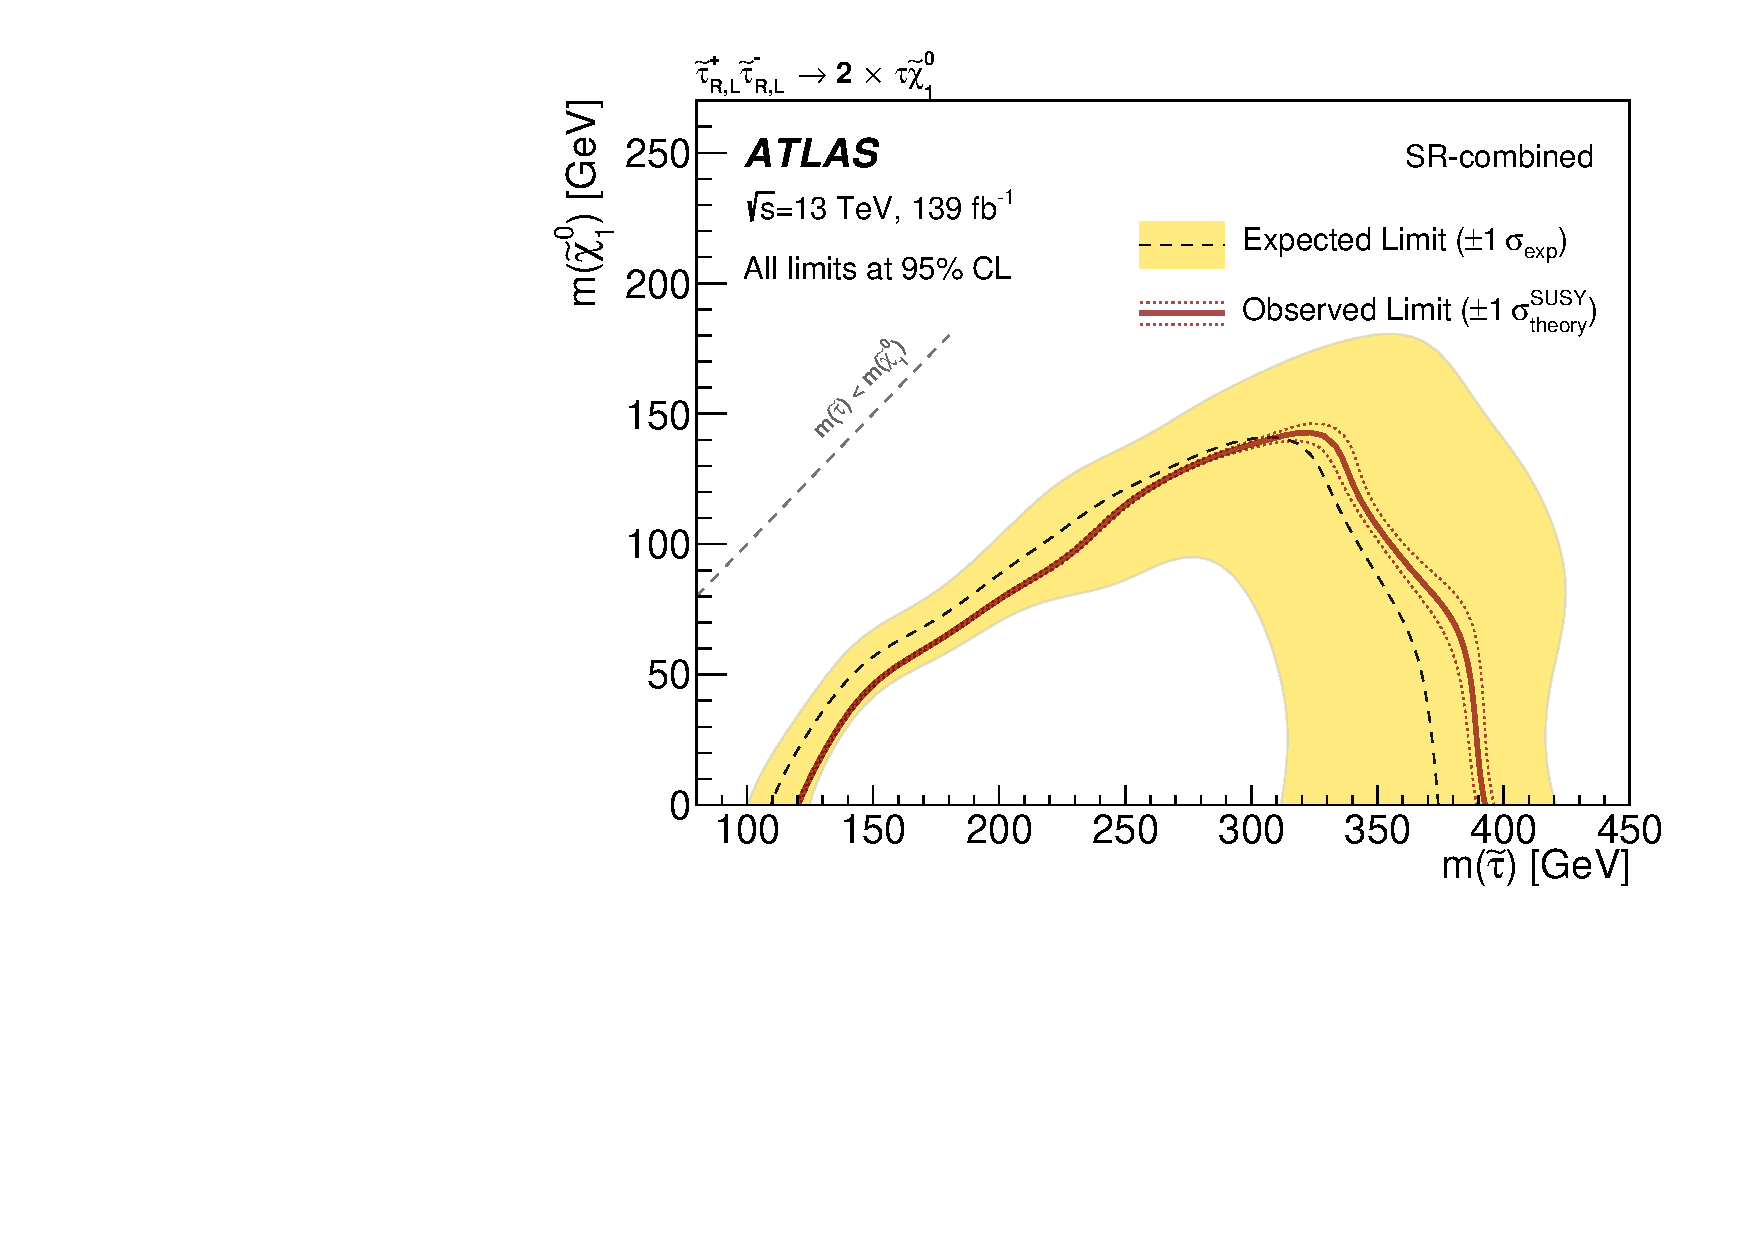
\includegraphics[width=0.5\textwidth]{beyondLHC/limit_DS_combine_EXP_staustau}\label{fig:exclusion_staustau}}
		 \subbottom[]{
			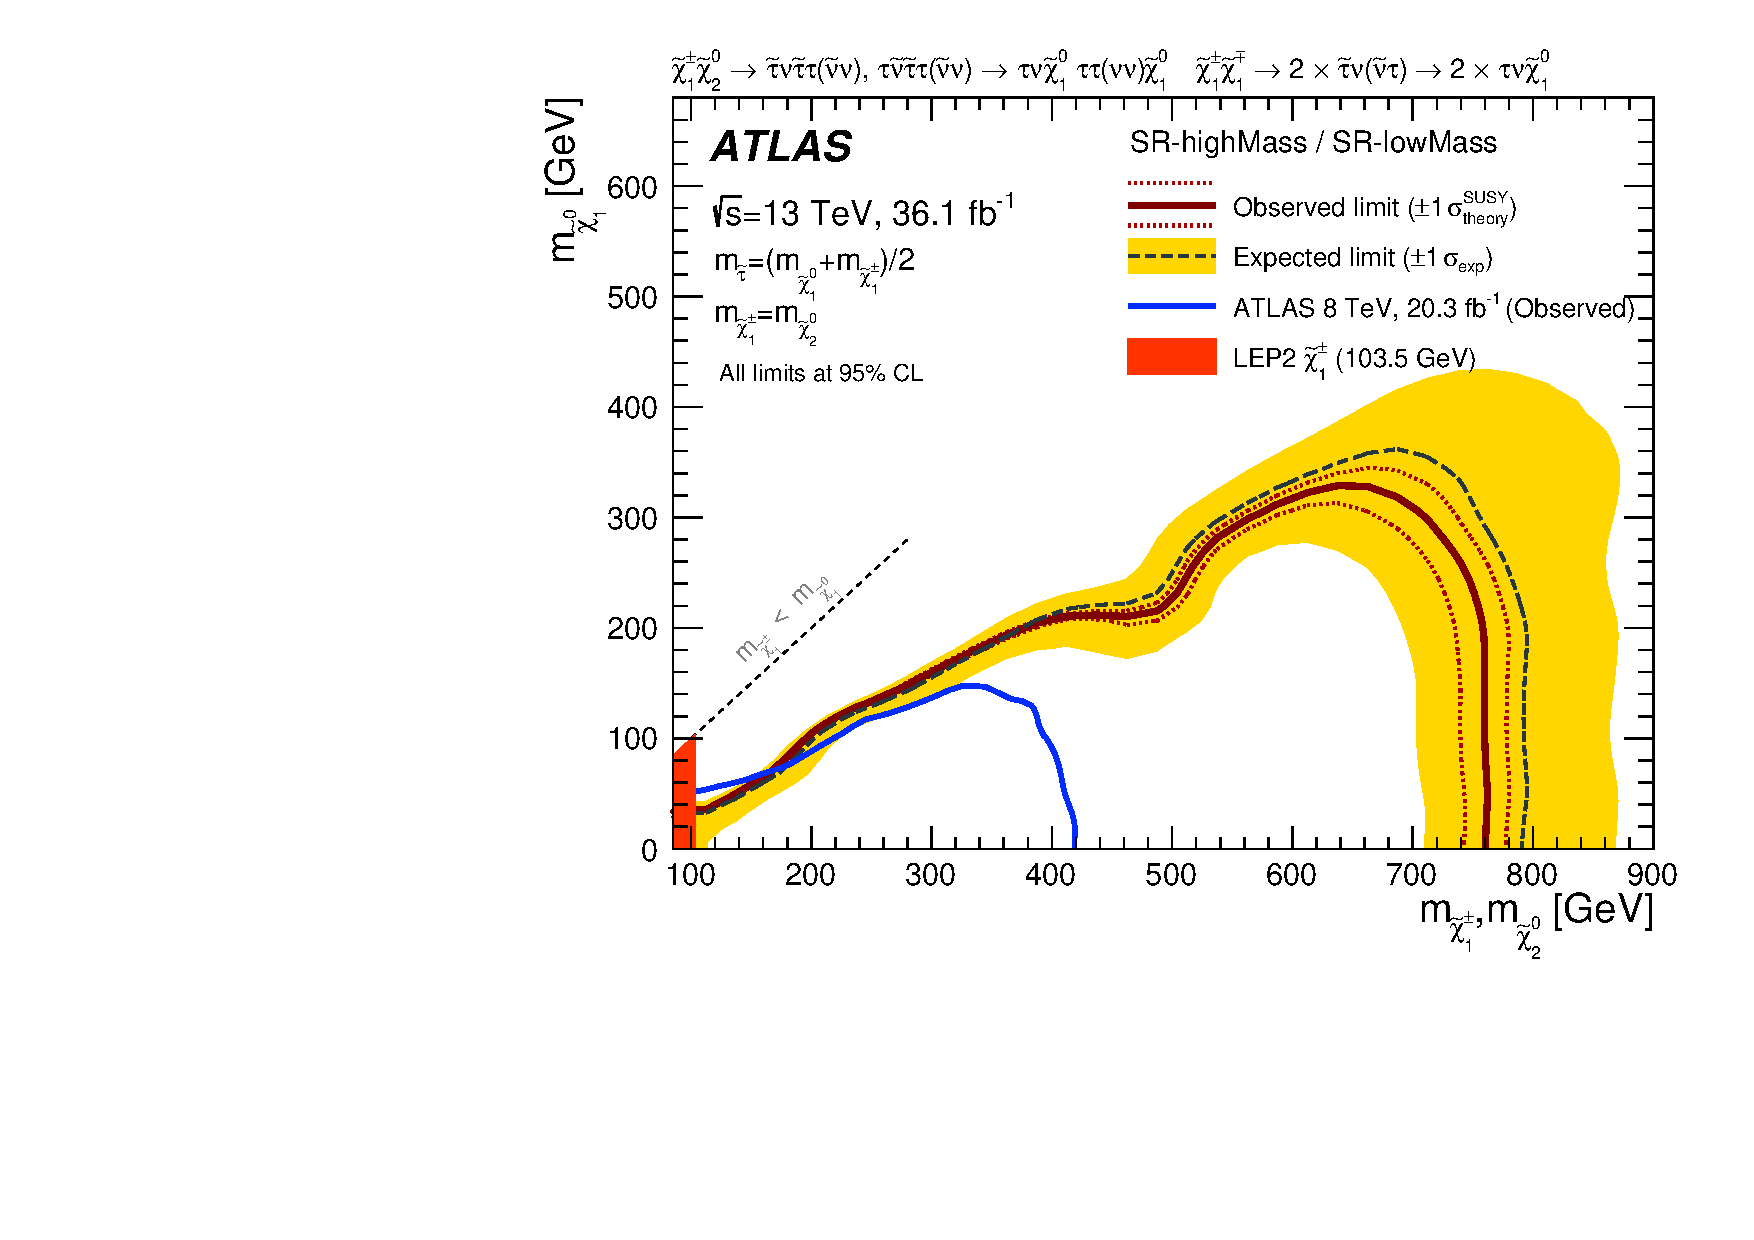
\includegraphics[width=0.45\textwidth]{beyondLHC/C1C1_C1N2_comb_exclusion}\label{fig:exclusion_c1n2_c1c1}}
	\end{center}
\caption{Observed and expected 95\% exclusion limits for simplified models with (a) direct \stau\  pair production, and (b) \chinoonepm\  and \ninoone\ production with \stau. Plots are produced using 139 \infb\ and 36.1 \infb\ of proton-proton collisions data collected at \com$=13$ \tev\ at the \ac{LHC} by the \ac{ATLAS} experiment, respectively.}
\label{fig:exclusion}
\end{figure}
}

\newcommand{\FeynmanDiagramsVBF}{
\begin{figure}[!hbt]
\begin{center}
		\subbottom[]{
			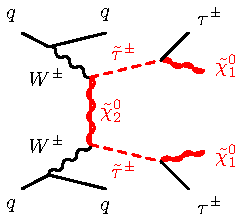
\includegraphics[width=0.3\textwidth]{beyondLHC/VBFstaustau}\label{fig:VBF_scenarios_a}}
		 \subbottom[]{
			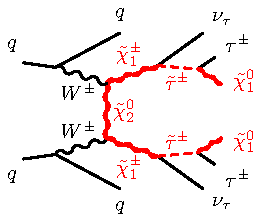
\includegraphics[width=0.3\textwidth]{beyondLHC/VBFC1C1staustau}\label{fig:VBF_scenarios_b}}
			 \subbottom[]{
			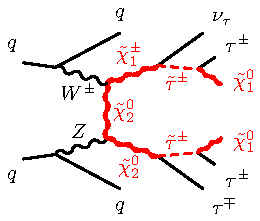
\includegraphics[width=0.3\textwidth]{beyondLHC/VBFC1N2staustau}\label{fig:VBF_scenarios_c}}
	\end{center}
\caption{Diagrams of the decay topology of the signal models considered in this chapter. Displayed processes show (a) the \ac{VBF} production of charged \stau\ with at least two associated jets, (b) the production of two \chinoonepm\  that further decay into \stau, and (c) the production of \chinoonepm\ and \ninotwo\ that further decay into \stau.}
\label{fig:VBF_scenarios}
\end{figure}
}

\newcommand{\NoSelectionAsymmetricTrigger}{
\begin{figure}[!hbt]
\begin{center}
	\subbottom[]{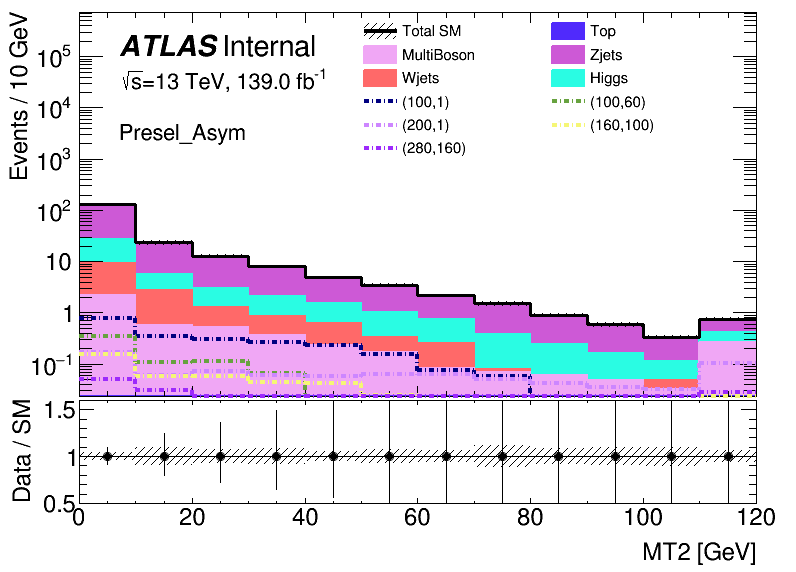
\includegraphics[width=0.45\textwidth]{beyondLHC/LowThresholdTriggers/Presel/Asym/MT2_max_Presel_Asym.png}}
%\subbottom[]{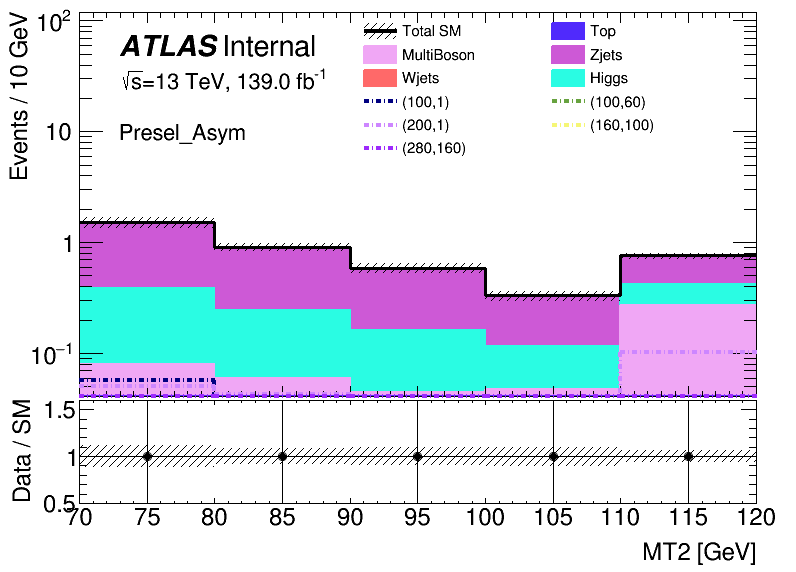
\includegraphics[width=0.45\textwidth]{beyondLHC/LowThresholdTriggers/Presel/Asym/MT2_max_SR_Presel_Asym.png}}
%\subbottom[]{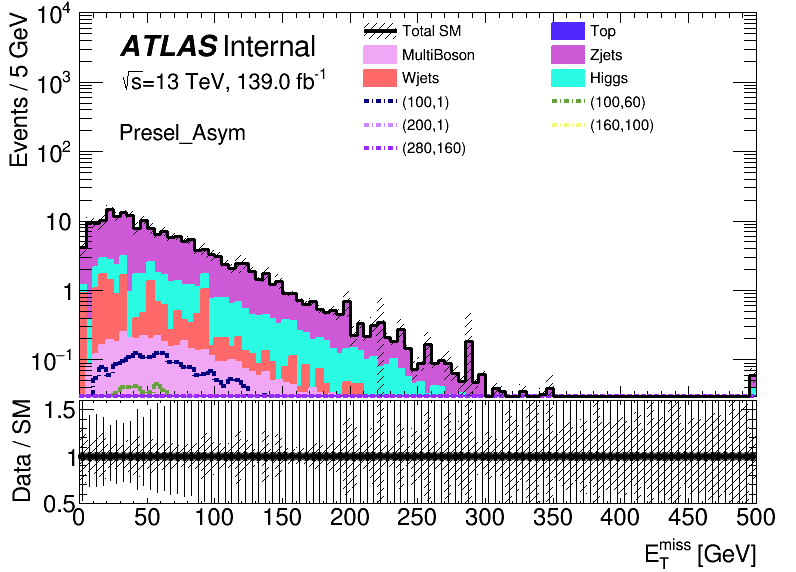
\includegraphics[width=0.45\textwidth]{beyondLHC/LowThresholdTriggers/Presel/Asym/MetTST_met_Presel_Asym.png}}
\subbottom[]{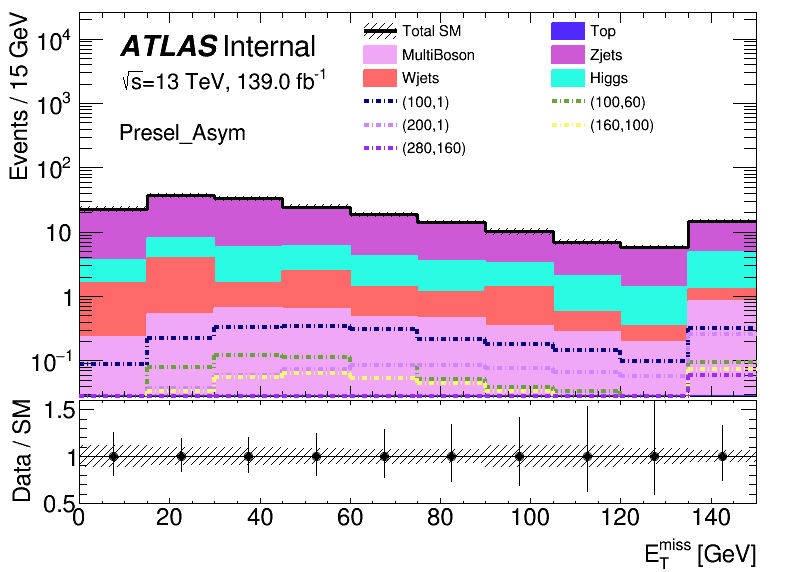
\includegraphics[width=0.45\textwidth]{beyondLHC/LowThresholdTriggers/Presel/Asym/MetTST_met_SR_Presel_Asym.png}}
%\subbottom[]{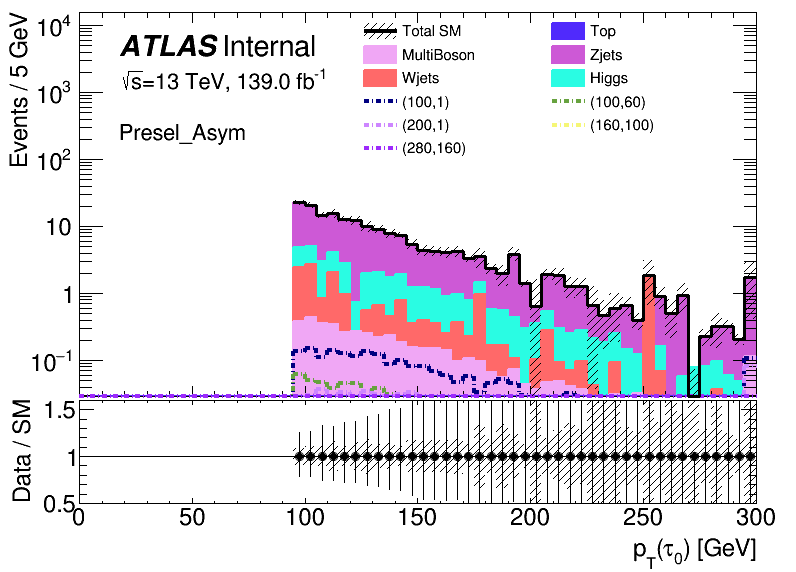
\includegraphics[width=0.45\textwidth]{beyondLHC/LowThresholdTriggers/Presel/Asym/leading_taus_pt_Presel_Asym.png}}
%\subbottom[]{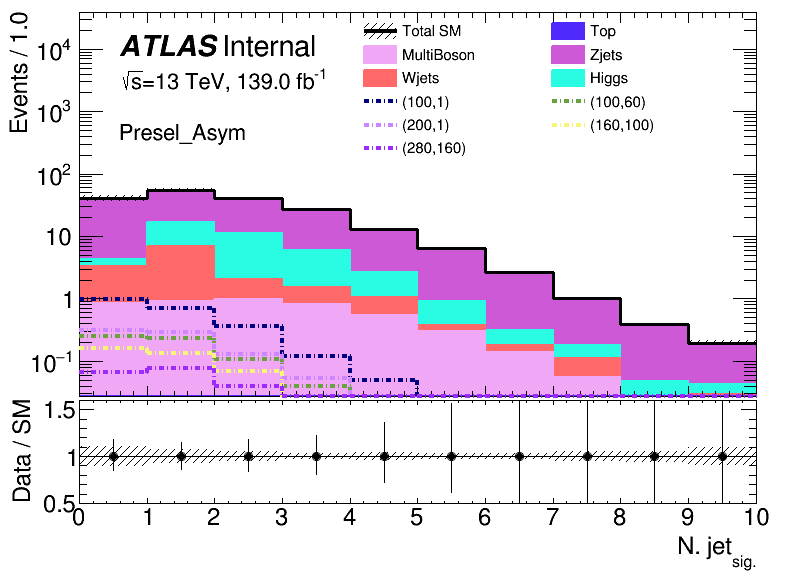
\includegraphics[width=0.45\textwidth]{beyondLHC/LowThresholdTriggers/Presel/Asym/n_SignalJets_Presel_Asym.png}}
%\subbottom[]{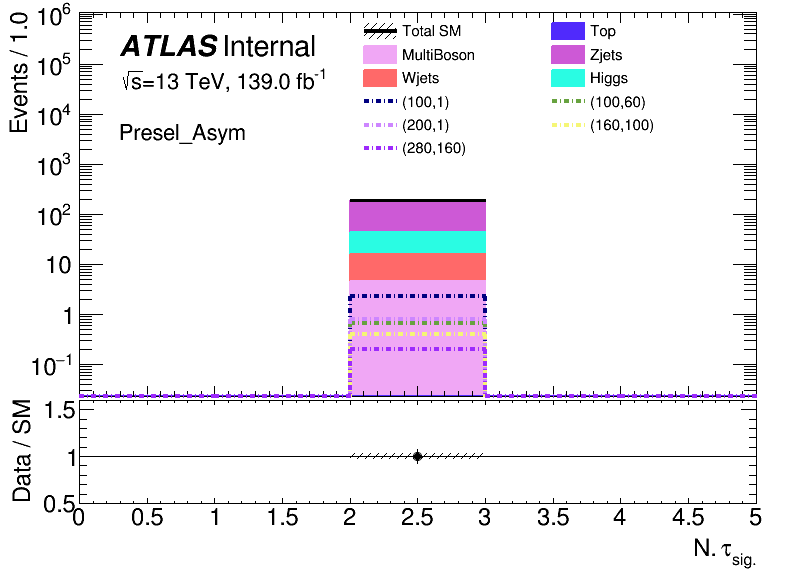
\includegraphics[width=0.45\textwidth]{beyondLHC/LowThresholdTriggers/Presel/Asym/n_SignalTau_Presel_Asym.png}}
%\subbottom[]{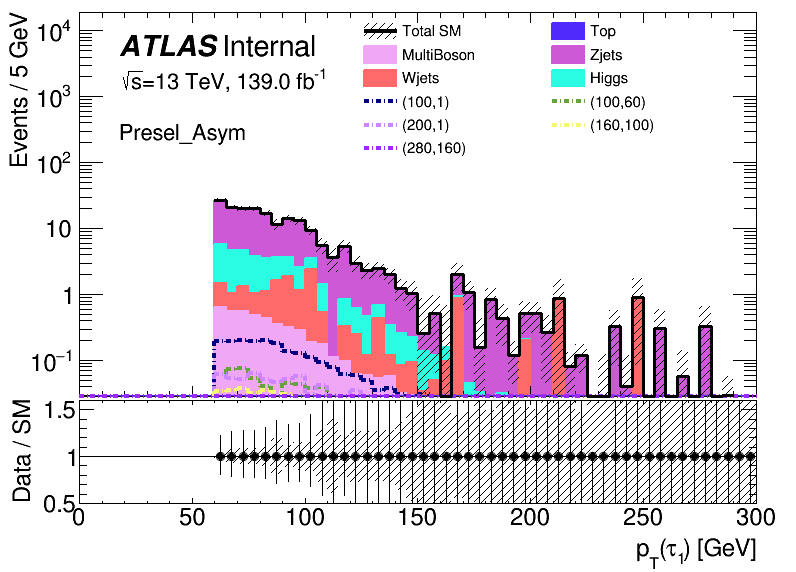
\includegraphics[width=0.45\textwidth]{beyondLHC/LowThresholdTriggers/Presel/Asym/subleading_taus_pt_Presel_Asym.png}}
%\subbottom[]{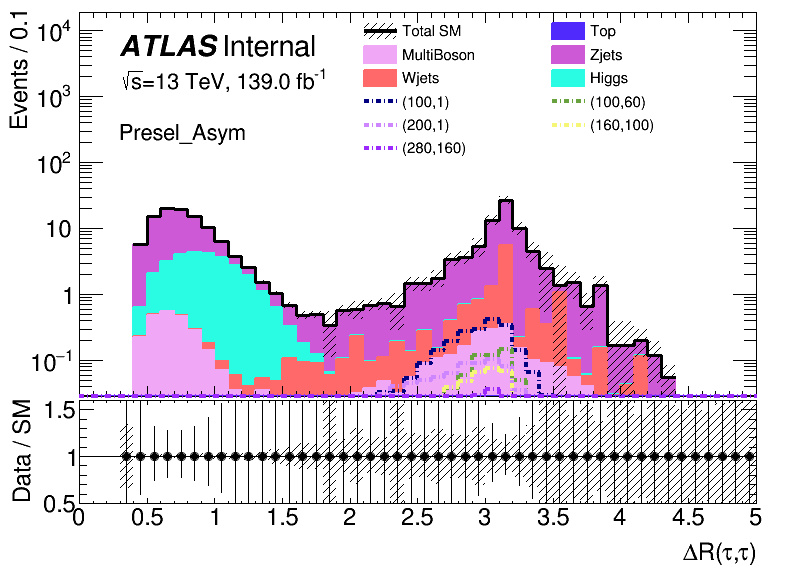
\includegraphics[width=0.45\textwidth]{beyondLHC/LowThresholdTriggers/Presel/Asym/taus_DR_Presel_Asym.png}}
%\subbottom[]{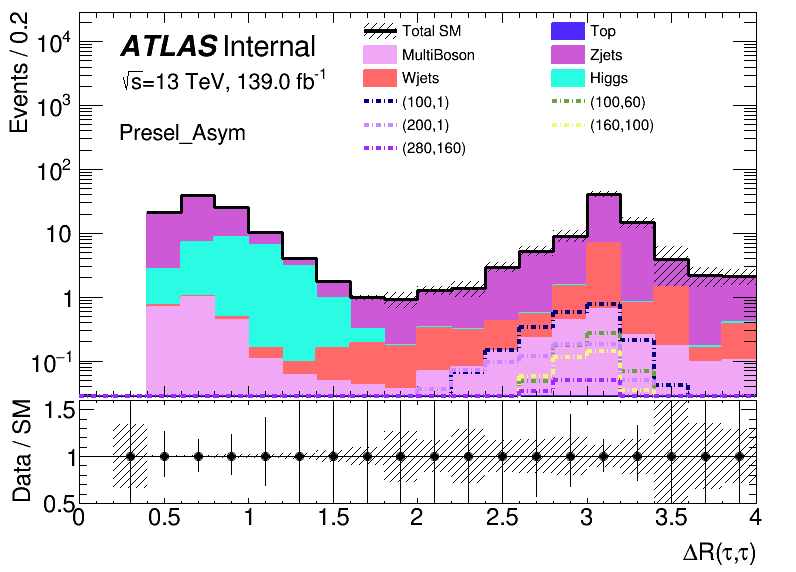
\includegraphics[width=0.45\textwidth]{beyondLHC/LowThresholdTriggers/Presel/Asym/taus_DR_SR_Presel_Asym.png}}
%\subbottom[]{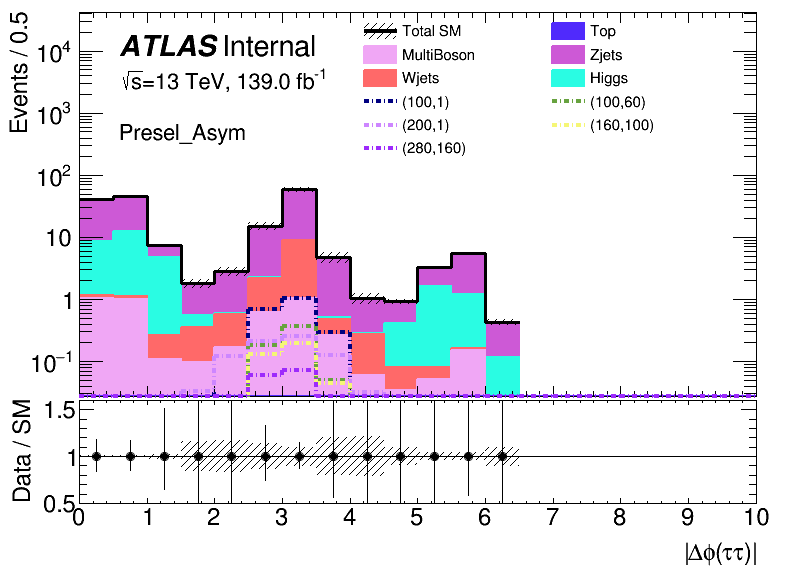
\includegraphics[width=0.45\textwidth]{beyondLHC/LowThresholdTriggers/Presel/Asym/taus_Dphi_Presel_Asym.png}}
%\subbottom[]{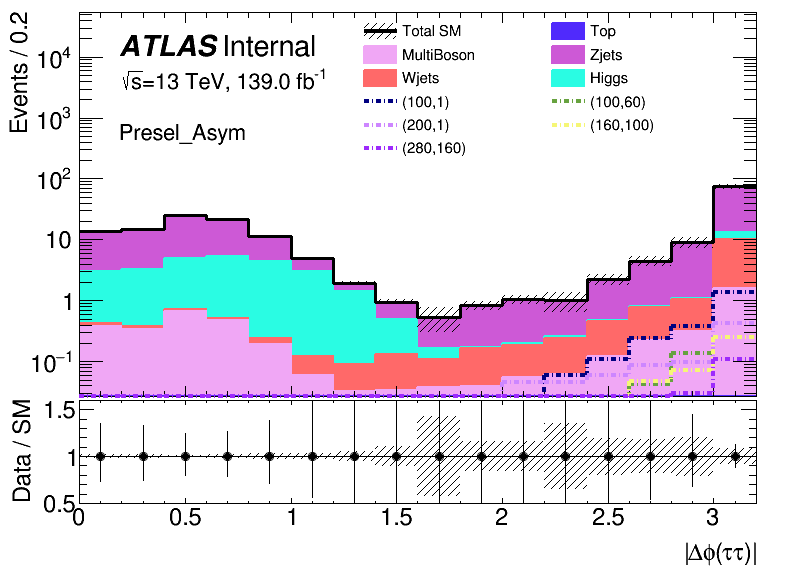
\includegraphics[width=0.45\textwidth]{beyondLHC/LowThresholdTriggers/Presel/Asym/taus_Dphi_SR_Presel_Asym.png}}
%\subbottom[]{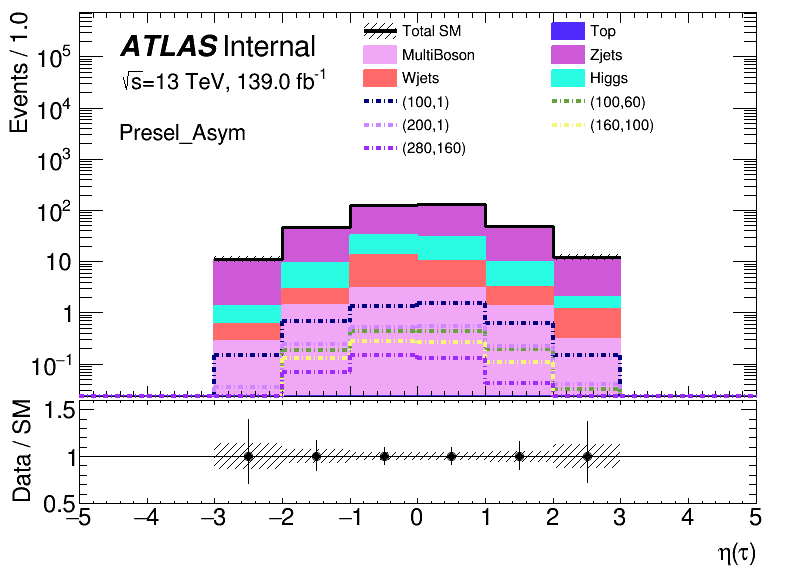
\includegraphics[width=0.45\textwidth]{beyondLHC/LowThresholdTriggers/Presel/Asym/taus_eta_Presel_Asym.png}}
\subbottom[]{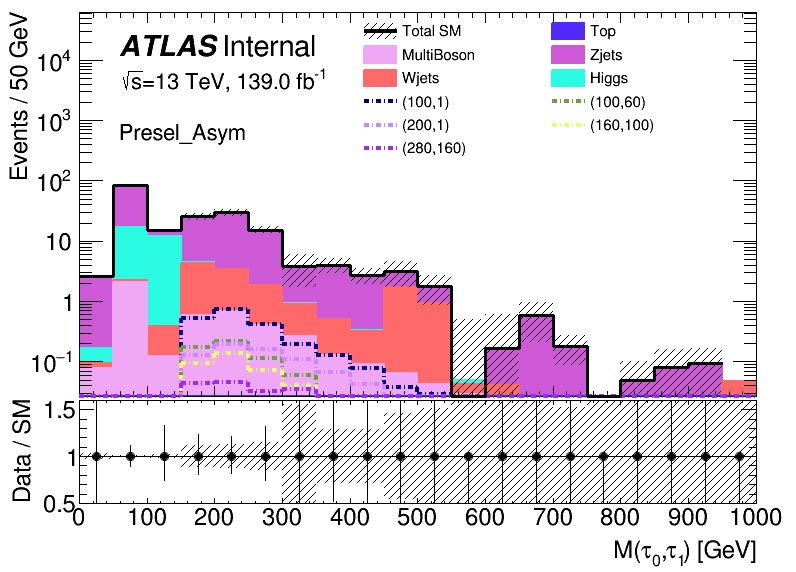
\includegraphics[width=0.45\textwidth]{beyondLHC/LowThresholdTriggers/Presel/Asym/taus_mtt_Presel_Asym.png}}
%\subbottom[]{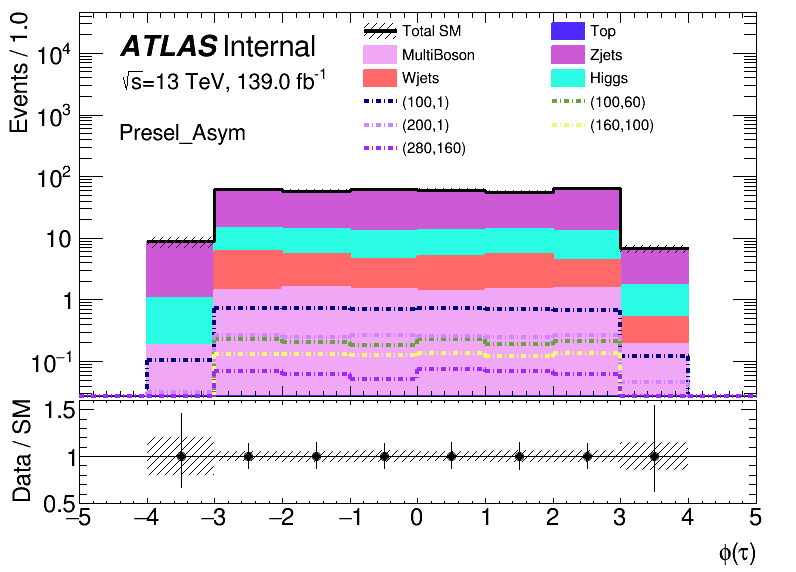
\includegraphics[width=0.45\textwidth]{beyondLHC/LowThresholdTriggers/Presel/Asym/taus_phi_Presel_Asym.png}}
\subbottom[]{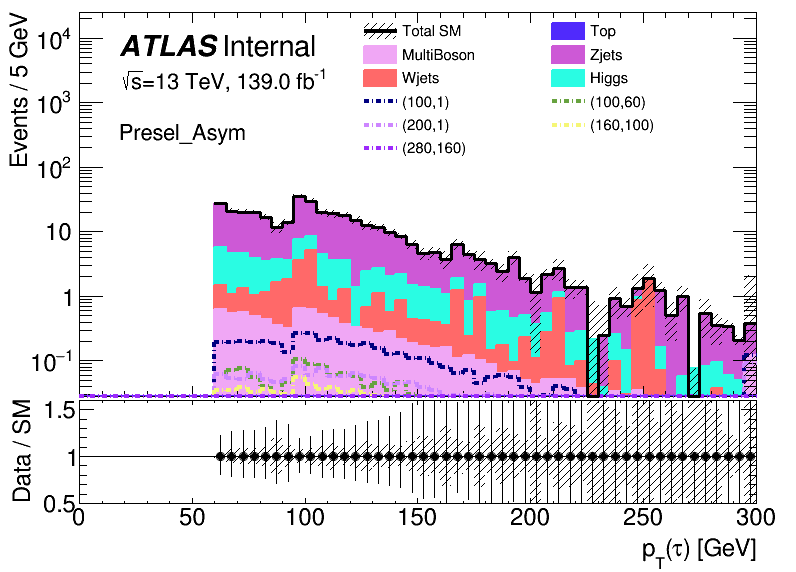
\includegraphics[width=0.45\textwidth]{beyondLHC/LowThresholdTriggers/Presel/Asym/taus_pt_Presel_Asym.png}}

\end{center}
\caption{Distributions of (a) MT2, (b) \met, (c) $M(\tau_0,\tau_1)$, and (d) $\pt(\tau)$ in the preselection region using the asymmetric di-tau trigger to select relevant events. Signal scenarios are shown by the dotted lines while \ac{SM} \ac{MC} samples displayed as stacked histogram. The shaded band include only systematic uncertainties in the background prediction.}
\label{fig:no_sel_asym}
\end{figure}
}

\newcommand{\NoSelectionFTTrigger}{
\begin{figure}[!hbt]
\begin{center}
\subbottom[]{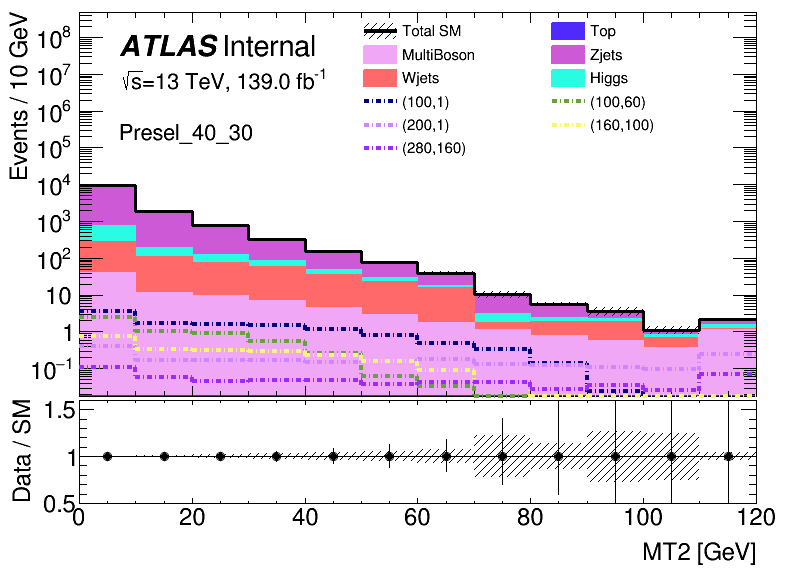
\includegraphics[width=0.45\textwidth]{beyondLHC/LowThresholdTriggers/Presel/4030/MT2_max_Presel_40_30.png}}
%\subbottom[]{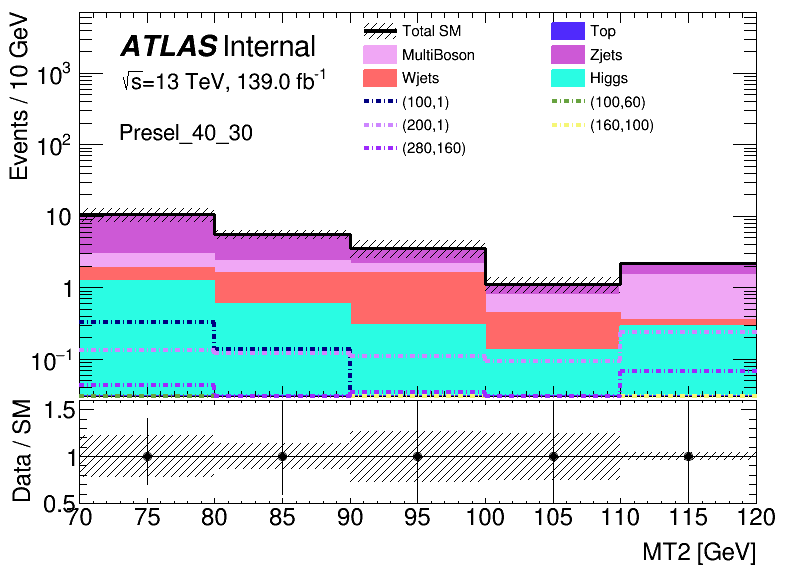
\includegraphics[width=0.45\textwidth]{beyondLHC/LowThresholdTriggers/Presel/4030/MT2_max_SR_Presel_40_30.png}}
%\subbottom[]{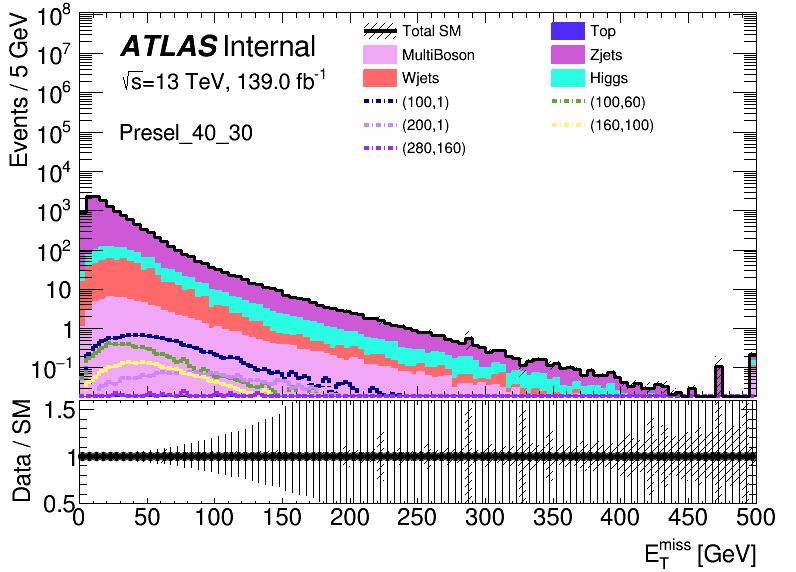
\includegraphics[width=0.45\textwidth]{beyondLHC/LowThresholdTriggers/Presel/4030/MetTST_met_Presel_40_30.png}}
\subbottom[]{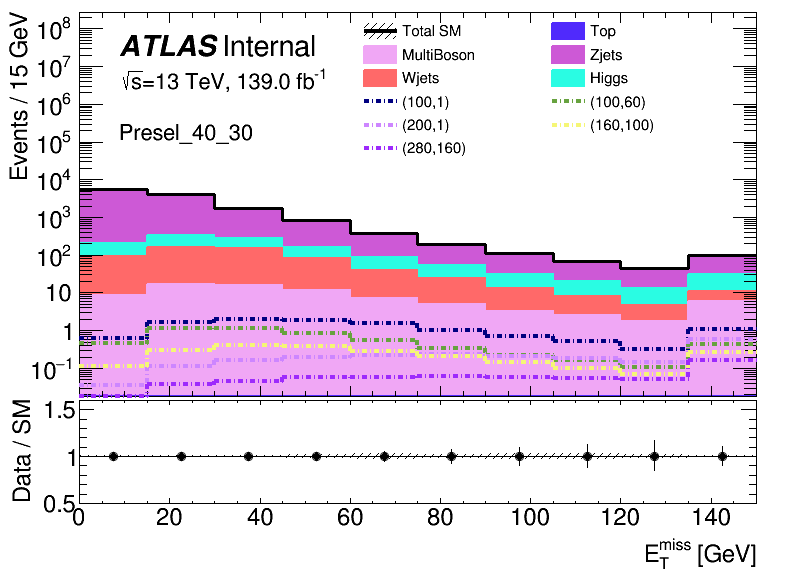
\includegraphics[width=0.45\textwidth]{beyondLHC/LowThresholdTriggers/Presel/4030/MetTST_met_SR_Presel_40_30.png}}
%\subbottom[]{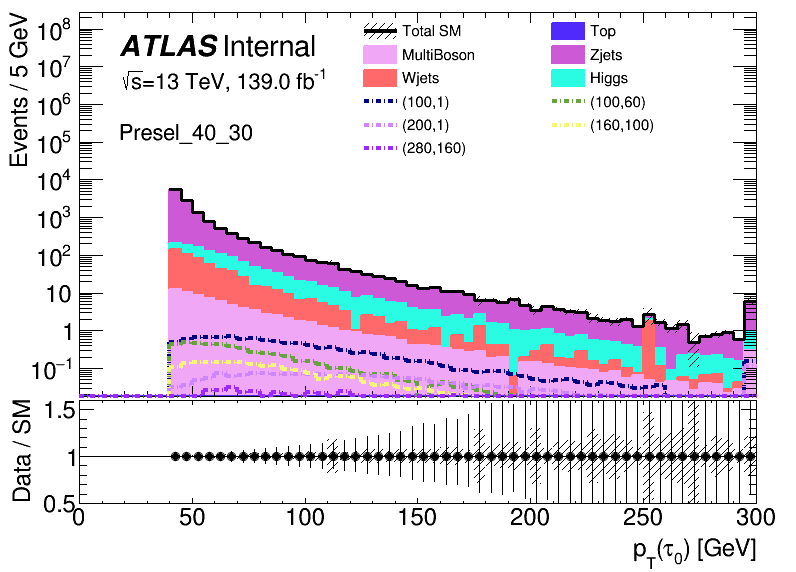
\includegraphics[width=0.45\textwidth]{beyondLHC/LowThresholdTriggers/Presel/4030/leading_taus_pt_Presel_40_30.png}}
%\subbottom[]{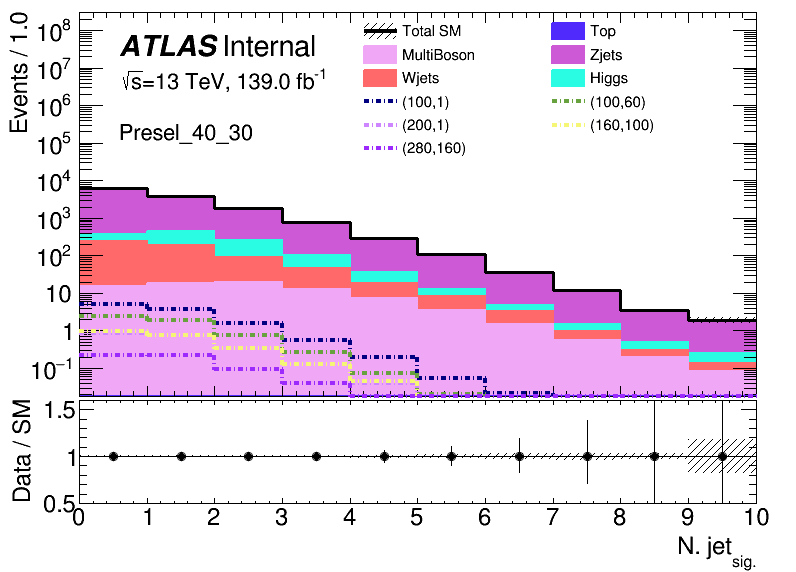
\includegraphics[width=0.45\textwidth]{beyondLHC/LowThresholdTriggers/Presel/4030/n_SignalJets_Presel_40_30.png}}
%\subbottom[]{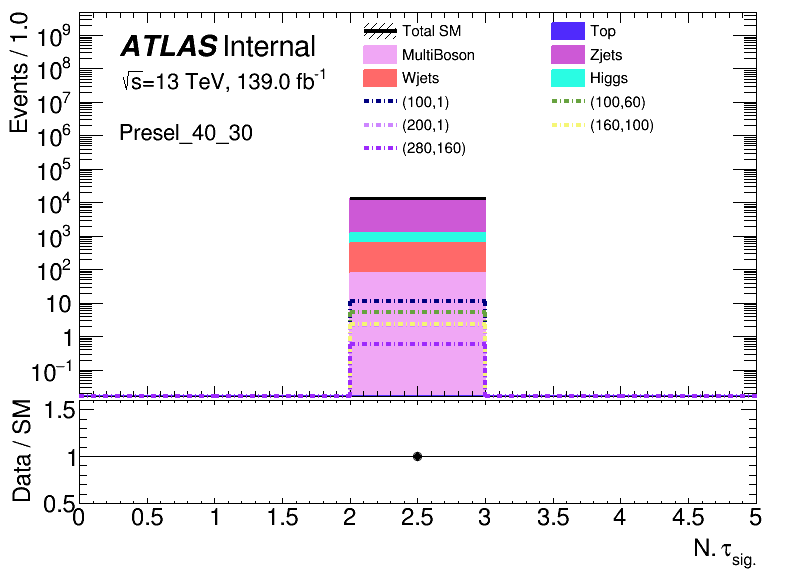
\includegraphics[width=0.45\textwidth]{beyondLHC/LowThresholdTriggers/Presel/4030/n_SignalTau_Presel_40_30.png}}
%\subbottom[]{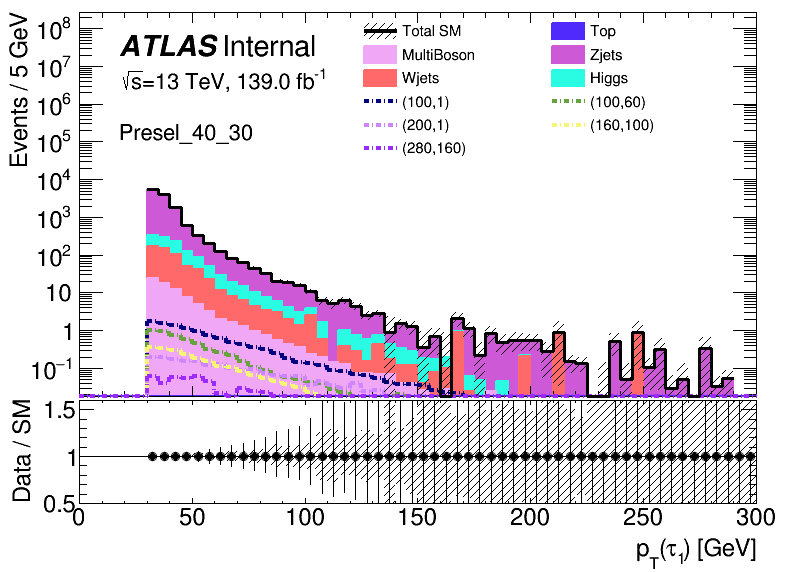
\includegraphics[width=0.45\textwidth]{beyondLHC/LowThresholdTriggers/Presel/4030/subleading_taus_pt_Presel_40_30.png}}
%\subbottom[]{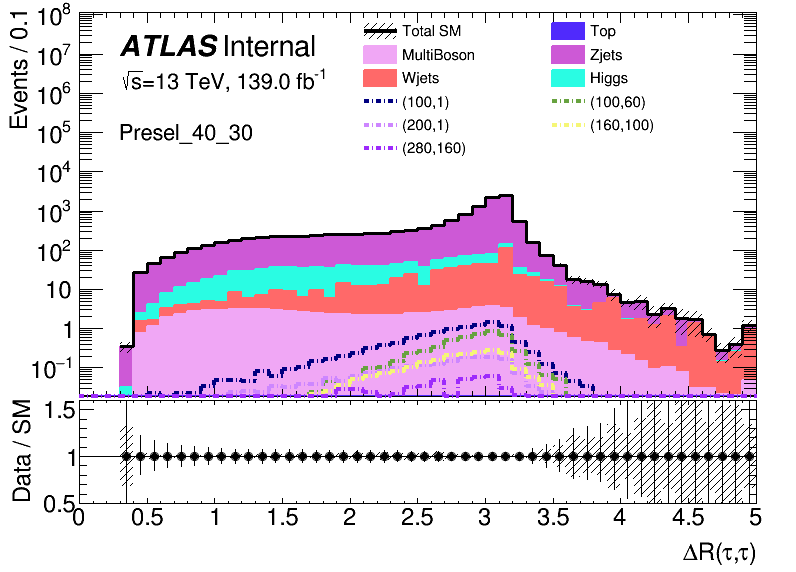
\includegraphics[width=0.45\textwidth]{beyondLHC/LowThresholdTriggers/Presel/4030/taus_DR_Presel_40_30.png}}
%\subbottom[]{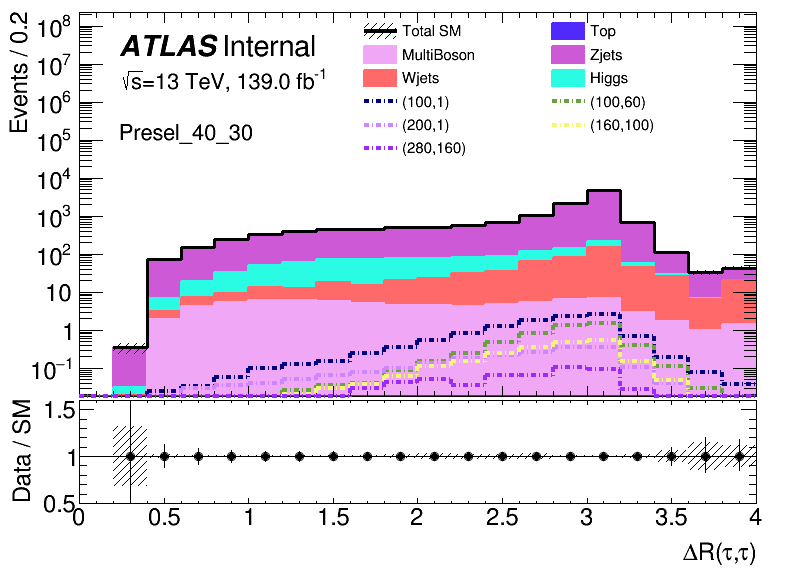
\includegraphics[width=0.45\textwidth]{beyondLHC/LowThresholdTriggers/Presel/4030/taus_DR_SR_Presel_40_30.png}}
%\subbottom[]{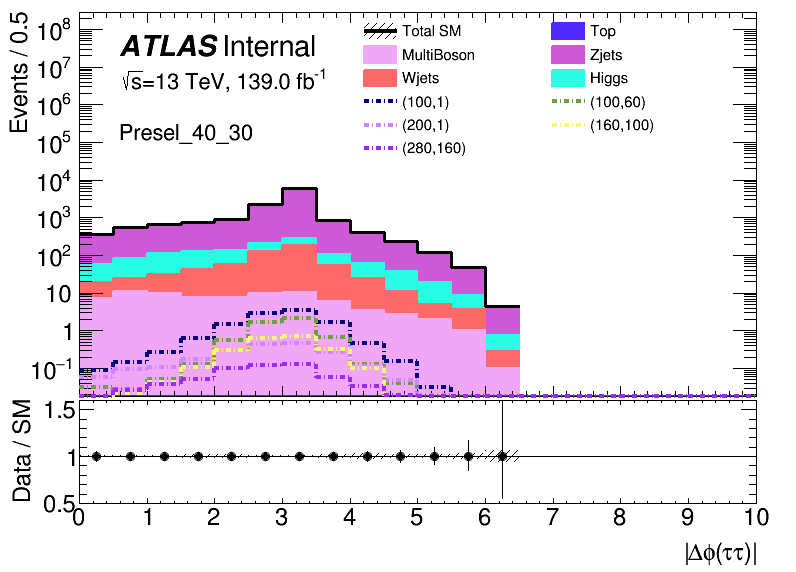
\includegraphics[width=0.45\textwidth]{beyondLHC/LowThresholdTriggers/Presel/4030/taus_Dphi_Presel_40_30.png}}
%\subbottom[]{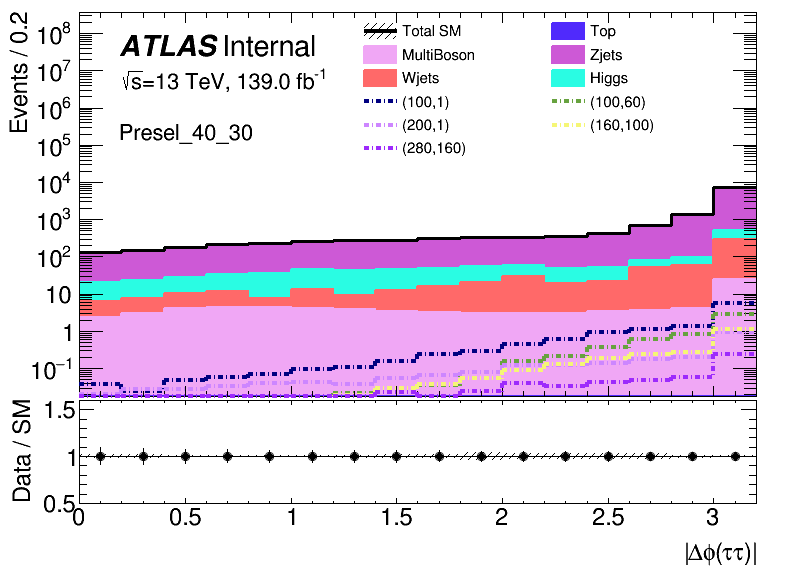
\includegraphics[width=0.45\textwidth]{beyondLHC/LowThresholdTriggers/Presel/4030/taus_Dphi_SR_Presel_40_30.png}}
%\subbottom[]{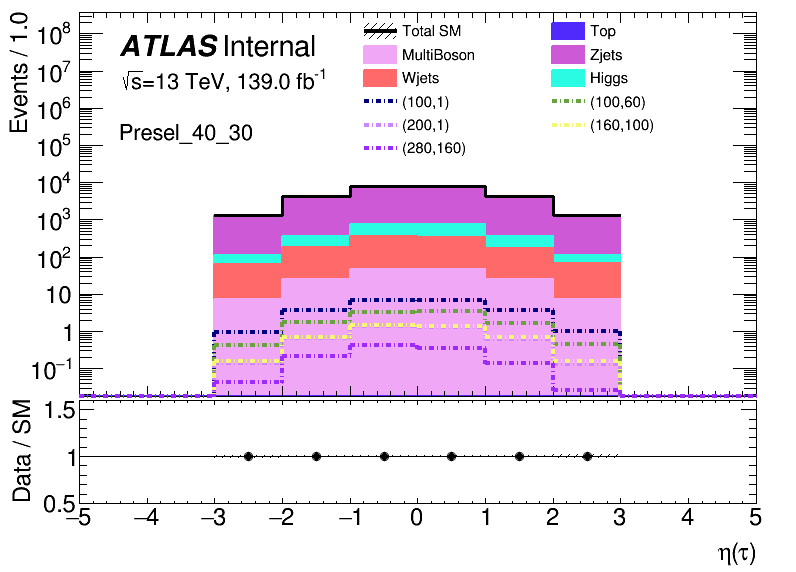
\includegraphics[width=0.45\textwidth]{beyondLHC/LowThresholdTriggers/Presel/4030/taus_eta_Presel_40_30.png}}
\subbottom[]{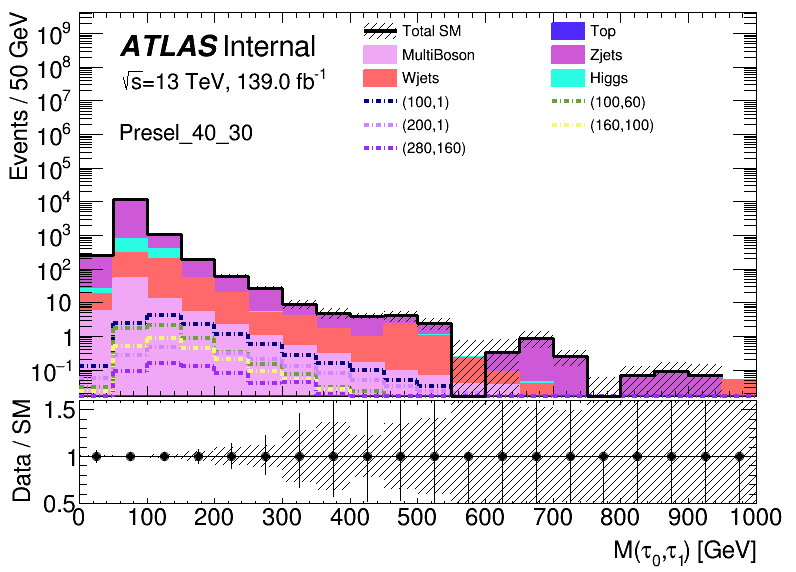
\includegraphics[width=0.45\textwidth]{beyondLHC/LowThresholdTriggers/Presel/4030/taus_mtt_Presel_40_30.png}}
%\subbottom[]{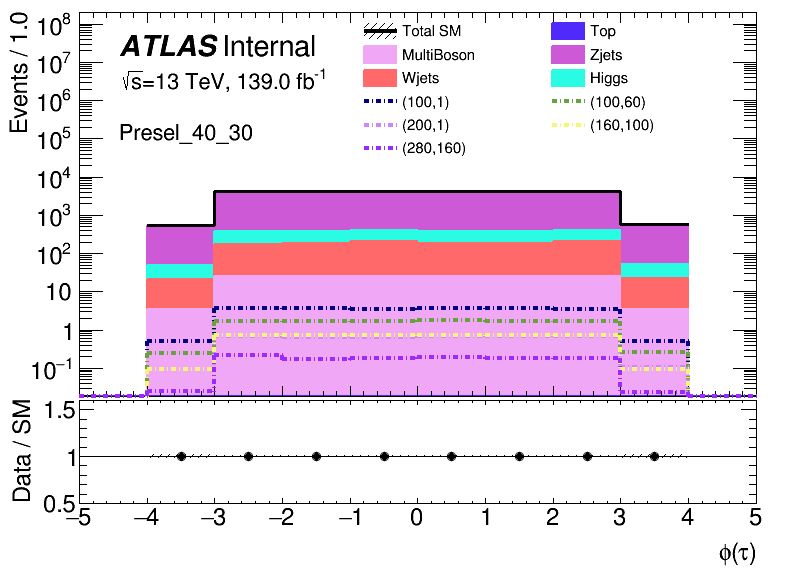
\includegraphics[width=0.45\textwidth]{beyondLHC/LowThresholdTriggers/Presel/4030/taus_phi_Presel_40_30.png}}
\subbottom[]{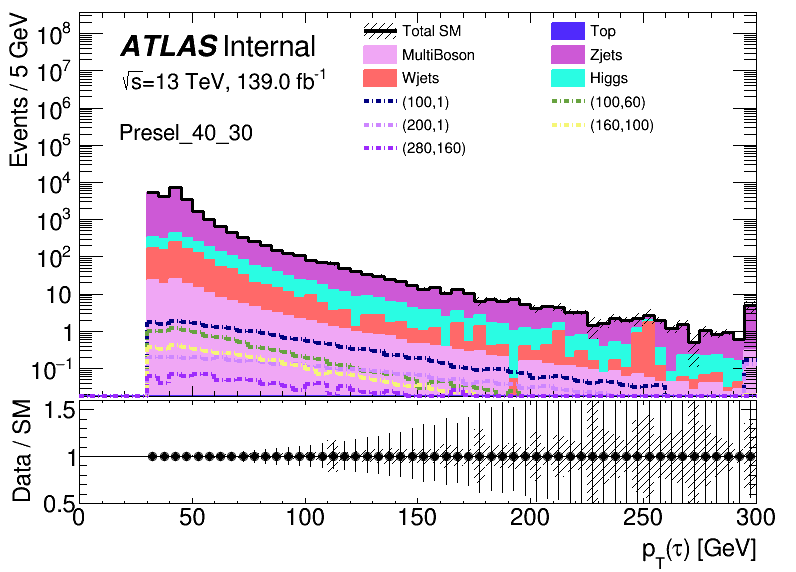
\includegraphics[width=0.45\textwidth]{beyondLHC/LowThresholdTriggers/Presel/4030/taus_pt_Presel_40_30.png}}

\end{center}
\caption{Distributions of (a) MT2, (b) \met, (c) $M(\tau_0,\tau_1)$, and (d) $\pt(\tau)$ in the preselection region using the lowered $\pt(\tau_0)>40$ \gev\ and $\pt(\tau_1)>30$ \gev\  offline thresholds to select relevant events. Signal scenarios are shown by the dotted lines while \ac{SM} \ac{MC} samples displayed as stacked histogram. The shaded band include only systematic uncertainties in the background prediction.}
\label{fig:no_sel_4030}
\end{figure}
}

\newcommand{\NoSelectionTTTrigger}{
\begin{figure}[!hbt]
\begin{center}
\subbottom[]{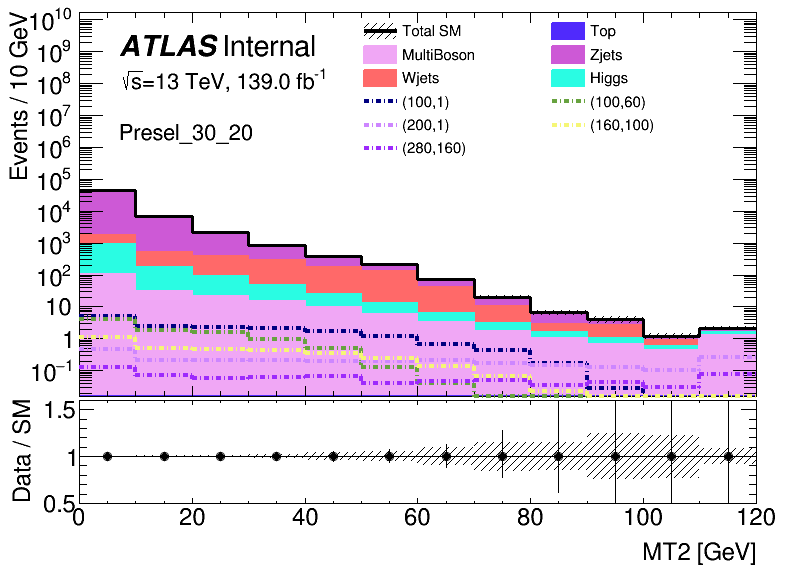
\includegraphics[width=0.45\textwidth]{beyondLHC/LowThresholdTriggers/Presel/3020/MT2_max_Presel_30_20.png}}
%\subbottom[]{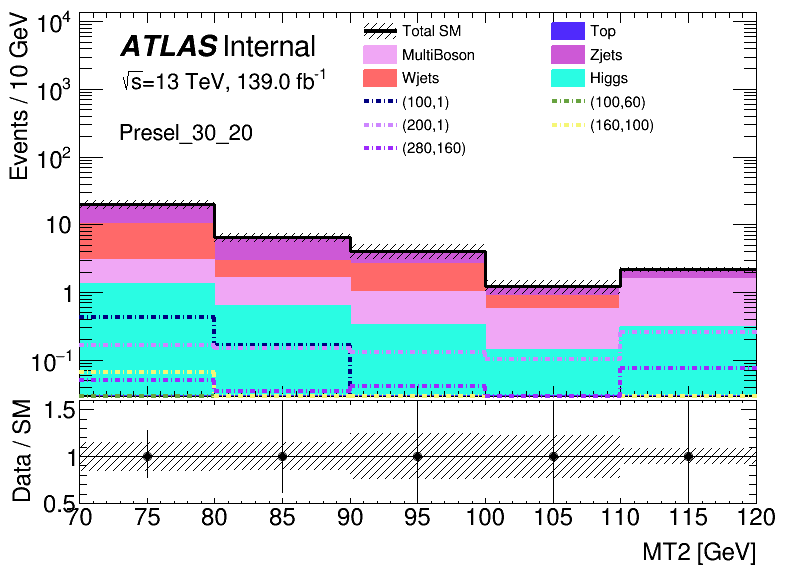
\includegraphics[width=0.45\textwidth]{beyondLHC/LowThresholdTriggers/Presel/3020/MT2_max_SR_Presel_30_20.png}}
%\subbottom[]{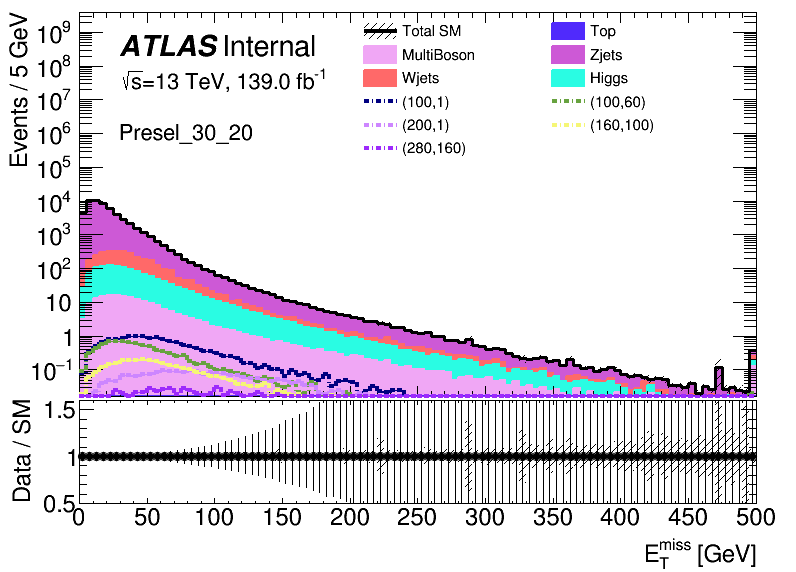
\includegraphics[width=0.45\textwidth]{beyondLHC/LowThresholdTriggers/Presel/3020/MetTST_met_Presel_30_20.png}}
\subbottom[]{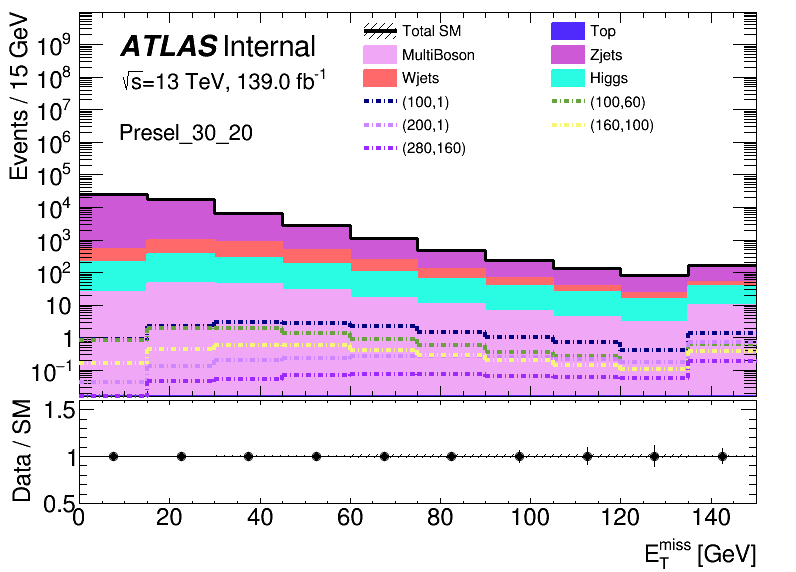
\includegraphics[width=0.45\textwidth]{beyondLHC/LowThresholdTriggers/Presel/3020/MetTST_met_SR_Presel_30_20.png}}
%\subbottom[]{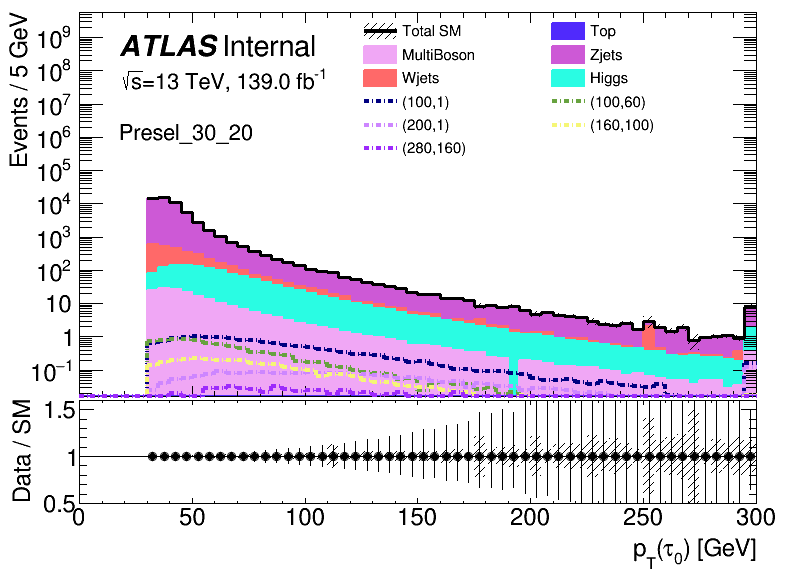
\includegraphics[width=0.45\textwidth]{beyondLHC/LowThresholdTriggers/Presel/3020/leading_taus_pt_Presel_30_20.png}}
%\subbottom[]{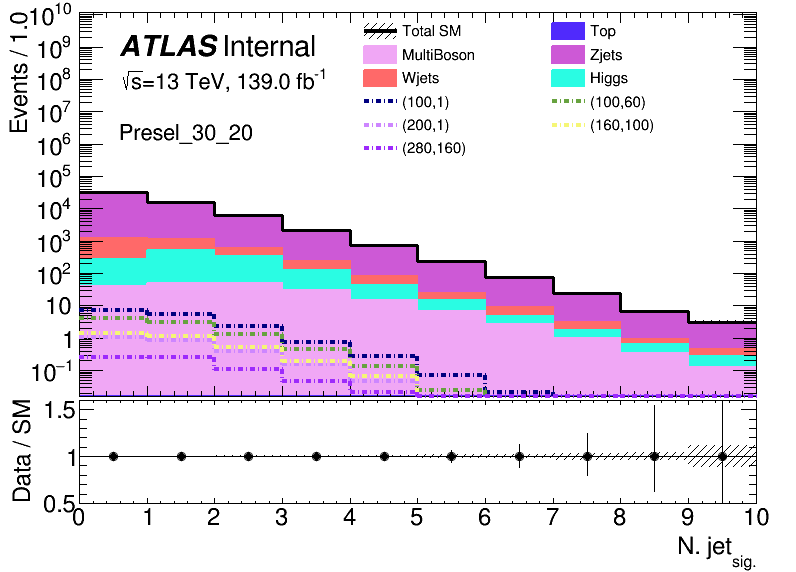
\includegraphics[width=0.45\textwidth]{beyondLHC/LowThresholdTriggers/Presel/3020/n_SignalJets_Presel_30_20.png}}
%\subbottom[]{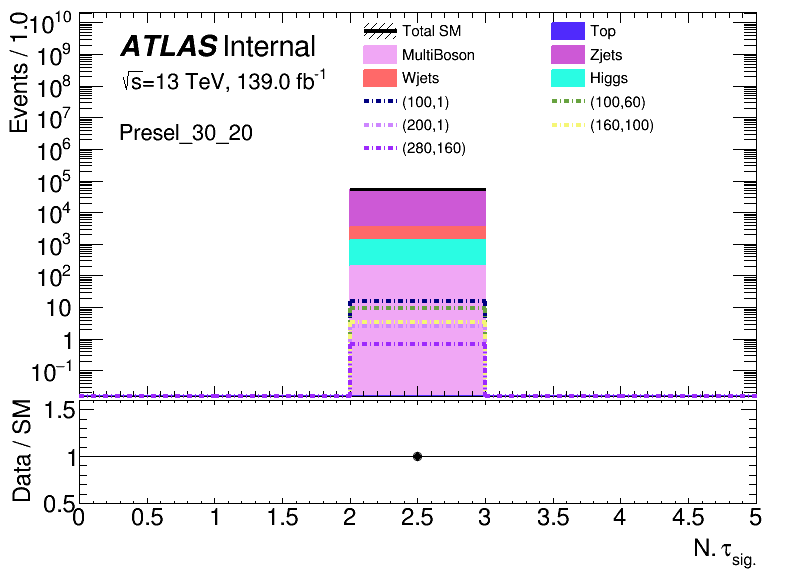
\includegraphics[width=0.45\textwidth]{beyondLHC/LowThresholdTriggers/Presel/3020/n_SignalTau_Presel_30_20.png}}
%\subbottom[]{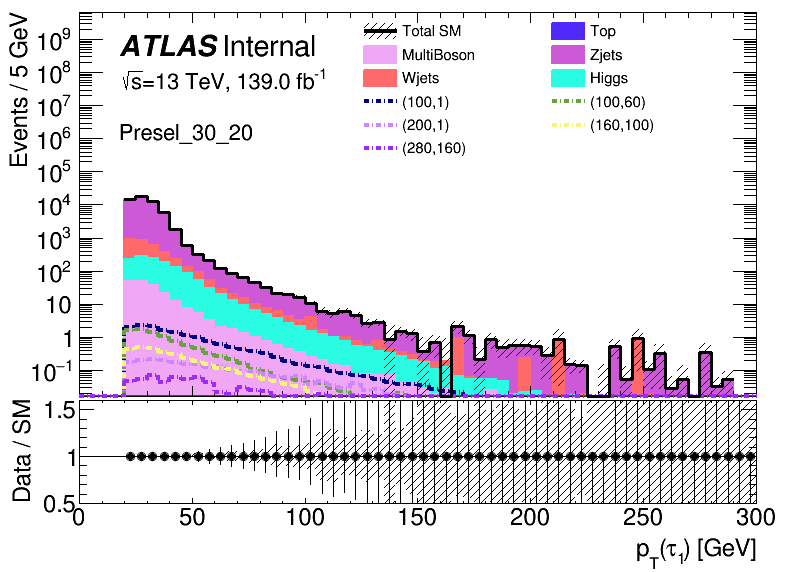
\includegraphics[width=0.45\textwidth]{beyondLHC/LowThresholdTriggers/Presel/3020/subleading_taus_pt_Presel_30_20.png}}
%\subbottom[]{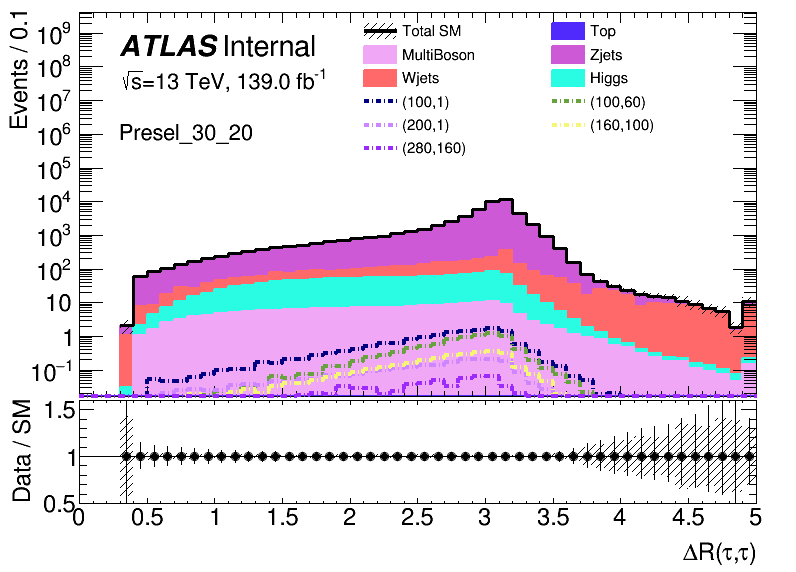
\includegraphics[width=0.45\textwidth]{beyondLHC/LowThresholdTriggers/Presel/3020/taus_DR_Presel_30_20.png}}
%\subbottom[]{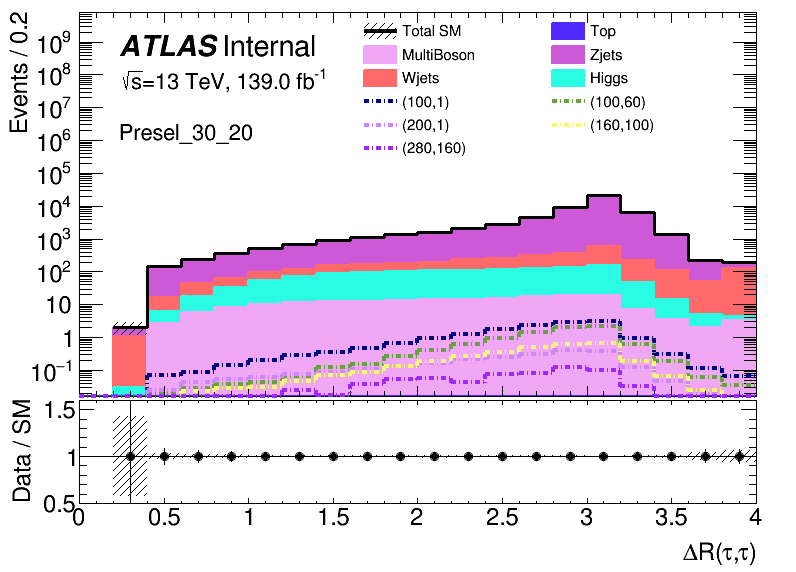
\includegraphics[width=0.45\textwidth]{beyondLHC/LowThresholdTriggers/Presel/3020/taus_DR_SR_Presel_30_20.png}}
%\subbottom[]{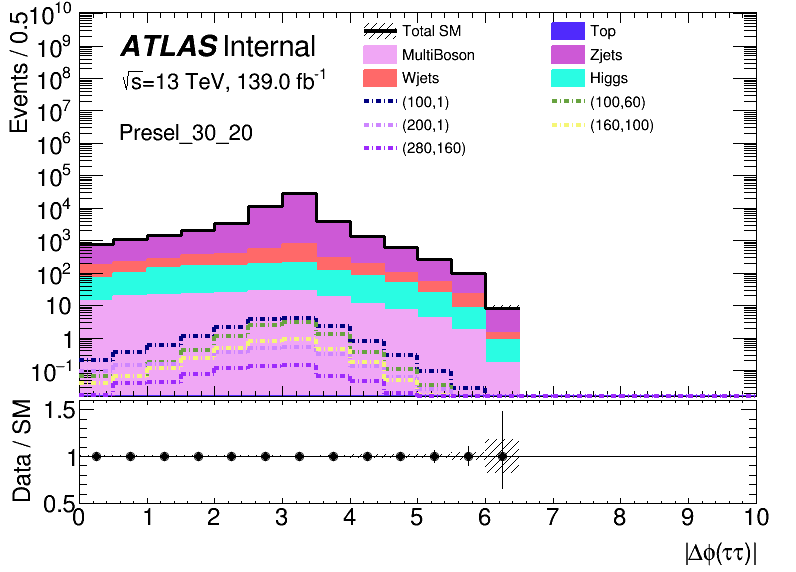
\includegraphics[width=0.45\textwidth]{beyondLHC/LowThresholdTriggers/Presel/3020/taus_Dphi_Presel_30_20.png}}
%\subbottom[]{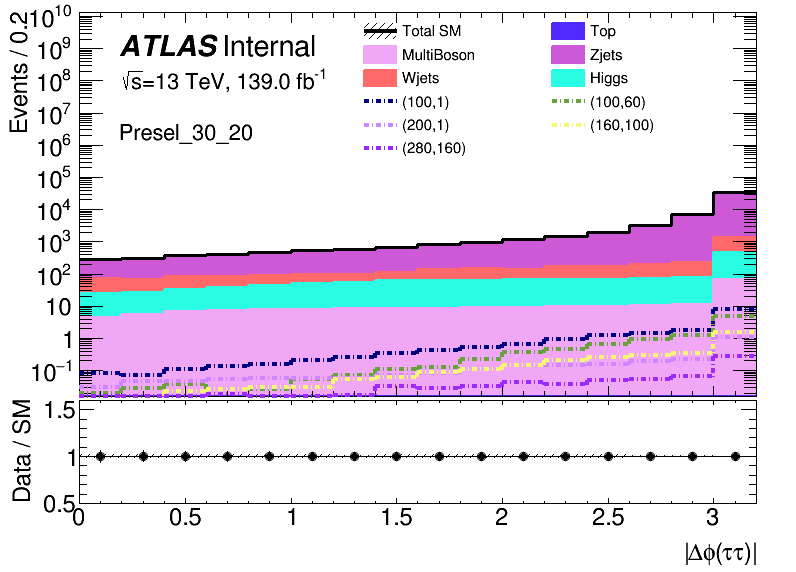
\includegraphics[width=0.45\textwidth]{beyondLHC/LowThresholdTriggers/Presel/3020/taus_Dphi_SR_Presel_30_20.png}}
%\subbottom[]{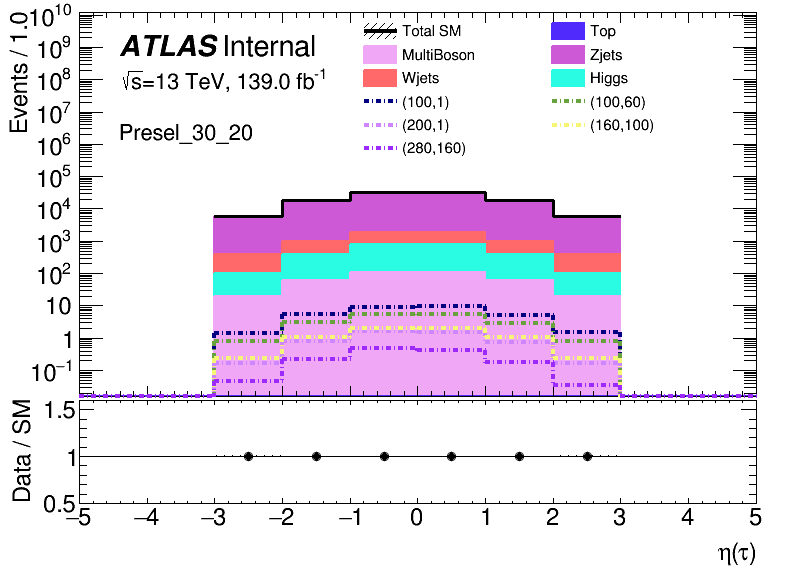
\includegraphics[width=0.45\textwidth]{beyondLHC/LowThresholdTriggers/Presel/3020/taus_eta_Presel_30_20.png}}
\subbottom[]{\includegraphics[width=0.45\textwidth]{beyondLHC/LowThresholdTriggers/Presel/3020/taus_mtt_Presel_30_20.png}}
%\subbottom[]{\includegraphics[width=0.45\textwidth]{beyondLHC/LowThresholdTriggers/Presel/3020/taus_phi_Presel_30_20.png}}
\subbottom[]{\includegraphics[width=0.45\textwidth]{beyondLHC/LowThresholdTriggers/Presel/3020/taus_pt_Presel_30_20.png}}

\end{center}
\caption{Distributions of (a) MT2, (b) \met, (c) $M(\tau_0,\tau_1)$, and (d) $\pt(\tau)$ in the preselection region using the lowered $\pt(\tau_0)>30$ \gev\ and $\pt(\tau_1)>20$ \gev\  offline thresholds to select relevant events. Signal scenarios are shown by the dotted lines while \ac{SM} \ac{MC} samples displayed as stacked histogram. The shaded band include only systematic uncertainties in the background prediction.}
\label{fig:no_sel_3020}
\end{figure}
}

%%%%
\newcommand{\SRAsymmetricTrigger}{
\begin{figure}[!hbt]
\begin{center}
	\subbottom[]{\includegraphics[width=0.45\textwidth]{beyondLHC/LowThresholdTriggers/SR/Asym/MT2_max_SR_Asym.png}}
%\subbottom[]{\includegraphics[width=0.45\textwidth]{beyondLHC/LowThresholdTriggers/SR/Asym/MT2_max_SR_SR_Asym.png}}
%\subbottom[]{\includegraphics[width=0.45\textwidth]{beyondLHC/LowThresholdTriggers/SR/Asym/MetTST_met_SR_Asym.png}}
\subbottom[]{\includegraphics[width=0.45\textwidth]{beyondLHC/LowThresholdTriggers/SR/Asym/MetTST_met_SR_SR_Asym.png}}
%\subbottom[]{\includegraphics[width=0.45\textwidth]{beyondLHC/LowThresholdTriggers/SR/Asym/leading_taus_pt_SR_Asym.png}}
%\subbottom[]{\includegraphics[width=0.45\textwidth]{beyondLHC/LowThresholdTriggers/SR/Asym/n_SignalJets_SR_Asym.png}}
%\subbottom[]{\includegraphics[width=0.45\textwidth]{beyondLHC/LowThresholdTriggers/SR/Asym/n_SignalTau_SR_Asym.png}}
%\subbottom[]{\includegraphics[width=0.45\textwidth]{beyondLHC/LowThresholdTriggers/SR/Asym/subleading_taus_pt_SR_Asym.png}}
%\subbottom[]{\includegraphics[width=0.45\textwidth]{beyondLHC/LowThresholdTriggers/SR/Asym/taus_DR_SR_Asym.png}}
%\subbottom[]{\includegraphics[width=0.45\textwidth]{beyondLHC/LowThresholdTriggers/SR/Asym/taus_DR_SR_SR_Asym.png}}
%\subbottom[]{\includegraphics[width=0.45\textwidth]{beyondLHC/LowThresholdTriggers/SR/Asym/taus_Dphi_SR_Asym.png}}
%\subbottom[]{\includegraphics[width=0.45\textwidth]{beyondLHC/LowThresholdTriggers/SR/Asym/taus_Dphi_SR_SR_Asym.png}}
%\subbottom[]{\includegraphics[width=0.45\textwidth]{beyondLHC/LowThresholdTriggers/SR/Asym/taus_eta_SR_Asym.png}}
\subbottom[]{\includegraphics[width=0.45\textwidth]{beyondLHC/LowThresholdTriggers/SR/Asym/taus_mtt_SR_Asym.png}}
%\subbottom[]{\includegraphics[width=0.45\textwidth]{beyondLHC/LowThresholdTriggers/SR/Asym/taus_phi_SR_Asym.png}}
\subbottom[]{\includegraphics[width=0.45\textwidth]{beyondLHC/LowThresholdTriggers/SR/Asym/taus_pt_SR_Asym.png}}
\end{center}
\caption{Distributions of (a) MT2, (b) \met, (c) $M(\tau_0,\tau_1)$, and (d) $\pt(\tau)$ in the \ac{SR} using the asymmetric di-tau trigger to select relevant events. Signal scenarios are shown by the dotted lines while \ac{SM} \ac{MC} samples displayed as stacked histogram. The shaded band include only systematic uncertainties in the background prediction.}
\label{fig:SR_sel_asym}
\end{figure}
}

\newcommand{\SRFTTrigger}{
\begin{figure}[!hbt]
\begin{center}
\subbottom[]{\includegraphics[width=0.45\textwidth]{beyondLHC/LowThresholdTriggers/SR/4030/MT2_max_SR_40_30.png}}
%\subbottom[]{\includegraphics[width=0.45\textwidth]{beyondLHC/LowThresholdTriggers/SR/4030/MT2_max_SR_SR_40_30.png}}
%\subbottom[]{\includegraphics[width=0.45\textwidth]{beyondLHC/LowThresholdTriggers/SR/4030/MetTST_met_SR_40_30.png}}
\subbottom[]{\includegraphics[width=0.45\textwidth]{beyondLHC/LowThresholdTriggers/SR/4030/MetTST_met_SR_SR_40_30.png}}
%\subbottom[]{\includegraphics[width=0.45\textwidth]{beyondLHC/LowThresholdTriggers/SR/4030/leading_taus_pt_SR_40_30.png}}
%\subbottom[]{\includegraphics[width=0.45\textwidth]{beyondLHC/LowThresholdTriggers/SR/4030/n_SignalJets_SR_40_30.png}}
%\subbottom[]{\includegraphics[width=0.45\textwidth]{beyondLHC/LowThresholdTriggers/SR/4030/n_SignalTau_SR_40_30.png}}
%\subbottom[]{\includegraphics[width=0.45\textwidth]{beyondLHC/LowThresholdTriggers/SR/4030/subleading_taus_pt_SR_40_30.png}}
%\subbottom[]{\includegraphics[width=0.45\textwidth]{beyondLHC/LowThresholdTriggers/SR/4030/taus_DR_SR_40_30.png}}
%\subbottom[]{\includegraphics[width=0.45\textwidth]{beyondLHC/LowThresholdTriggers/SR/4030/taus_DR_SR_SR_40_30.png}}
%\subbottom[]{\includegraphics[width=0.45\textwidth]{beyondLHC/LowThresholdTriggers/SR/4030/taus_Dphi_SR_40_30.png}}
%\subbottom[]{\includegraphics[width=0.45\textwidth]{beyondLHC/LowThresholdTriggers/SR/4030/taus_Dphi_SR_SR_40_30.png}}
%\subbottom[]{\includegraphics[width=0.45\textwidth]{beyondLHC/LowThresholdTriggers/SR/4030/taus_eta_SR_40_30.png}}
\subbottom[]{\includegraphics[width=0.45\textwidth]{beyondLHC/LowThresholdTriggers/SR/4030/taus_mtt_SR_40_30.png}}
%\subbottom[]{\includegraphics[width=0.45\textwidth]{beyondLHC/LowThresholdTriggers/SR/4030/taus_phi_SR_40_30.png}}
\subbottom[]{\includegraphics[width=0.45\textwidth]{beyondLHC/LowThresholdTriggers/SR/4030/taus_pt_SR_40_30.png}}
\end{center}
\caption{Distributions of (a) MT2, (b) \met, (c) $M(\tau_0,\tau_1)$, and (d) $\pt(\tau)$ in the \ac{SR} using the lowered $\pt(\tau_0)>40$ \gev\ and $\pt(\tau_1)>30$ \gev\  offline thresholds to select relevant events. Signal scenarios are shown by the dotted lines while \ac{SM} \ac{MC} samples displayed as stacked histogram. The shaded band include only systematic uncertainties in the background prediction.}
\label{fig:SR_sel_4030}
\end{figure}
}

\newcommand{\SRTTTrigger}{
\begin{figure}[!hbt]
\begin{center}
\subbottom[]{\includegraphics[width=0.45\textwidth]{beyondLHC/LowThresholdTriggers/SR/3020/MT2_max_SR_30_20.png}}
%\subbottom[]{\includegraphics[width=0.45\textwidth]{beyondLHC/LowThresholdTriggers/SR/3020/MT2_max_SR_SR_30_20.png}}
%\subbottom[]{\includegraphics[width=0.45\textwidth]{beyondLHC/LowThresholdTriggers/SR/3020/MetTST_met_SR_30_20.png}}
\subbottom[]{\includegraphics[width=0.45\textwidth]{beyondLHC/LowThresholdTriggers/SR/3020/MetTST_met_SR_SR_30_20.png}}
%\subbottom[]{\includegraphics[width=0.45\textwidth]{beyondLHC/LowThresholdTriggers/SR/3020/leading_taus_pt_SR_30_20.png}}
%\subbottom[]{\includegraphics[width=0.45\textwidth]{beyondLHC/LowThresholdTriggers/SR/3020/n_SignalJets_SR_30_20.png}}
%\subbottom[]{\includegraphics[width=0.45\textwidth]{beyondLHC/LowThresholdTriggers/SR/3020/n_SignalTau_SR_30_20.png}}
%\subbottom[]{\includegraphics[width=0.45\textwidth]{beyondLHC/LowThresholdTriggers/SR/3020/subleading_taus_pt_SR_30_20.png}}
%\subbottom[]{\includegraphics[width=0.45\textwidth]{beyondLHC/LowThresholdTriggers/SR/3020/taus_DR_SR_30_20.png}}
%\subbottom[]{\includegraphics[width=0.45\textwidth]{beyondLHC/LowThresholdTriggers/SR/3020/taus_DR_SR_SR_30_20.png}}
%\subbottom[]{\includegraphics[width=0.45\textwidth]{beyondLHC/LowThresholdTriggers/SR/3020/taus_Dphi_SR_30_20.png}}
%\subbottom[]{\includegraphics[width=0.45\textwidth]{beyondLHC/LowThresholdTriggers/SR/3020/taus_Dphi_SR_SR_30_20.png}}
%\subbottom[]{\includegraphics[width=0.45\textwidth]{beyondLHC/LowThresholdTriggers/SR/3020/taus_eta_SR_30_20.png}}
\subbottom[]{\includegraphics[width=0.45\textwidth]{beyondLHC/LowThresholdTriggers/SR/3020/taus_mtt_SR_30_20.png}}
%\subbottom[]{\includegraphics[width=0.45\textwidth]{beyondLHC/LowThresholdTriggers/SR/3020/taus_phi_SR_30_20.png}}
\subbottom[]{\includegraphics[width=0.45\textwidth]{beyondLHC/LowThresholdTriggers/SR/3020/taus_pt_SR_30_20.png}}
\end{center}
\caption{Distributions of (a) MT2, (b) \met, (c) $M(\tau_0,\tau_1)$, and (d) $\pt(\tau)$ in the \ac{SR} using the lowered $\pt(\tau_0)>30$ \gev\ and $\pt(\tau_1)>20$ \gev\  offline thresholds to select relevant events. Signal scenarios are shown by the dotted lines while \ac{SM} \ac{MC} samples displayed as stacked histogram. The shaded band include only systematic uncertainties in the background prediction.}
\label{fig:SR_sel_3020}
\end{figure}
}
%%%


\newcommand{\VBFCCNoSelection}{
\begin{figure}[!hbt]
\begin{center}
\subbottom[]{\includegraphics[width=0.3\textwidth]{beyondLHC/C1N2_C1C1/C1C1/NoSelection/tau_eta_VBFC1N2_NoSelection.png}}
\subbottom[]{\includegraphics[width=0.3\textwidth]{beyondLHC/C1N2_C1C1/C1C1/NoSelection/tau_phi_VBFC1N2_NoSelection.png}}
\subbottom[]{\includegraphics[width=0.3\textwidth]{beyondLHC/C1N2_C1C1/C1C1/NoSelection/tau_pt_VBFC1N2_NoSelection.png}}
\subbottom[]{\includegraphics[width=0.3\textwidth]{beyondLHC/C1N2_C1C1/C1C1/NoSelection/N_baselineTaus_VBFC1N2_NoSelection.png}}
\subbottom[]{\includegraphics[width=0.3\textwidth]{beyondLHC/C1N2_C1C1/C1C1/NoSelection/N_goodJets_VBFC1N2_NoSelection.png}}
\subbottom[]{\includegraphics[width=0.3\textwidth]{beyondLHC/C1N2_C1C1/C1C1/NoSelection/eT_miss_CMS_VBFC1N2_NoSelection.png}}
\subbottom[]{\includegraphics[width=0.3\textwidth]{beyondLHC/C1N2_C1C1/C1C1/NoSelection/JetEta_VBFC1N2_NoSelection.png}}
\subbottom[]{\includegraphics[width=0.3\textwidth]{beyondLHC/C1N2_C1C1/C1C1/NoSelection/JetPhi_VBFC1N2_NoSelection.png}}
\subbottom[]{\includegraphics[width=0.3\textwidth]{beyondLHC/C1N2_C1C1/C1C1/NoSelection/JetPt_VBFC1N2_NoSelection.png}}
\subbottom[]{\includegraphics[width=0.3\textwidth]{beyondLHC/C1N2_C1C1/C1C1/NoSelection/MT2_VBFC1N2_NoSelection.png}}
%\subbottom[]{\includegraphics[width=0.3\textwidth]{beyondLHC/C1N2_C1C1/C1C1/NoSelection/eT_miss_VBFC1N2_NoSelection.png}}
%\subbottom[]{\includegraphics[width=0.3\textwidth]{beyondLHC/C1N2_C1C1/C1C1/NoSelection/jet_DRjet_VBFC1N2_NoSelection.png}}
%\subbottom[]{\includegraphics[width=0.3\textwidth]{beyondLHC/C1N2_C1C1/C1C1/NoSelection/jet_DRtau_VBFC1N2_NoSelection.png}}
%\subbottom[]{\includegraphics[width=0.3\textwidth]{beyondLHC/C1N2_C1C1/C1C1/NoSelection/jet_detaj0j1_VBFC1N2_NoSelection.png}}
%\subbottom[]{\includegraphics[width=0.3\textwidth]{beyondLHC/C1N2_C1C1/C1C1/NoSelection/jet_detajj2_VBFC1N2_NoSelection.png}}
\subbottom[]{\includegraphics[width=0.3\textwidth]{beyondLHC/C1N2_C1C1/C1C1/NoSelection/jet_detajj_VBFC1N2_NoSelection.png}}
%\subbottom[]{\includegraphics[width=0.3\textwidth]{beyondLHC/C1N2_C1C1/C1C1/NoSelection/jet_dphij0j1_VBFC1N2_NoSelection.png}}
%\subbottom[]{\includegraphics[width=0.3\textwidth]{beyondLHC/C1N2_C1C1/C1C1/NoSelection/jet_dphijj_VBFC1N2_NoSelection.png}}
\subbottom[]{\includegraphics[width=0.3\textwidth]{beyondLHC/C1N2_C1C1/C1C1/NoSelection/jet_mjj_CMS_VBFC1N2_NoSelection.png}}
%\subbottom[]{\includegraphics[width=0.3\textwidth]{beyondLHC/C1N2_C1C1/C1C1/NoSelection/jet_mjj_VBFC1N2_NoSelection.png}}
%\subbottom[]{\includegraphics[width=0.3\textwidth]{beyondLHC/C1N2_C1C1/C1C1/NoSelection/jet_opposite_hemispherejj_VBFC1N2_NoSelection.png}}
%\subbottom[]{\includegraphics[width=0.3\textwidth]{beyondLHC/C1N2_C1C1/C1C1/NoSelection/tau_DRtau_VBFC1N2_NoSelection.png}}
%\subbottom[]{\includegraphics[width=0.3\textwidth]{beyondLHC/C1N2_C1C1/C1C1/NoSelection/tau_MT_VBFC1N2_NoSelection.png}}
%\subbottom[]{\includegraphics[width=0.3\textwidth]{beyondLHC/C1N2_C1C1/C1C1/NoSelection/tau_MTtau_VBFC1N2_NoSelection.png}}
%\subbottom[]{\includegraphics[width=0.3\textwidth]{beyondLHC/C1N2_C1C1/C1C1/NoSelection/tau_deta_VBFC1N2_NoSelection.png}}
%\subbottom[]{\includegraphics[width=0.3\textwidth]{beyondLHC/C1N2_C1C1/C1C1/NoSelection/tau_dphi_VBFC1N2_NoSelection.png}}
%\subbottom[]{\includegraphics[width=0.3\textwidth]{beyondLHC/C1N2_C1C1/C1C1/NoSelection/tau_eta0eta1_VBFC1N2_NoSelection.png}}
\end{center}
\caption{Distributions of (a) MT2, (b) \met, (c) $M(\tau_0,\tau_1)$, and (d) $\pt(\tau)$ in the \ac{SR} using the lowered $\pt(\tau_0)>30$ \gev\ and $\pt(\tau_1)>20$ \gev\  offline thresholds to select relevant events. Signal scenarios are shown by the dotted lines while \ac{SM} \ac{MC} samples displayed as stacked histogram. The shaded band include only systematic uncertainties in the background prediction.}
\label{fig:VBF_C1C1_nosel}
\end{figure}
}

\newcommand{\VBFCCSR}{
\begin{figure}[!hbt]
\begin{center}
\subbottom[]{\includegraphics[width=0.3\textwidth]{beyondLHC/C1N2_C1C1/C1C1/SR/tau_eta_VBFC1N2.png}}
\subbottom[]{\includegraphics[width=0.3\textwidth]{beyondLHC/C1N2_C1C1/C1C1/SR/tau_phi_VBFC1N2.png}}
\subbottom[]{\includegraphics[width=0.3\textwidth]{beyondLHC/C1N2_C1C1/C1C1/SR/tau_pt_VBFC1N2.png}}
\subbottom[]{\includegraphics[width=0.3\textwidth]{beyondLHC/C1N2_C1C1/C1C1/SR/N_baselineTaus_VBFC1N2.png}}
\subbottom[]{\includegraphics[width=0.3\textwidth]{beyondLHC/C1N2_C1C1/C1C1/SR/N_goodJets_VBFC1N2.png}}
\subbottom[]{\includegraphics[width=0.3\textwidth]{beyondLHC/C1N2_C1C1/C1C1/SR/eT_miss_CMS_VBFC1N2.png}}
\subbottom[]{\includegraphics[width=0.3\textwidth]{beyondLHC/C1N2_C1C1/C1C1/SR/JetEta_VBFC1N2.png}}
\subbottom[]{\includegraphics[width=0.3\textwidth]{beyondLHC/C1N2_C1C1/C1C1/SR/JetPhi_VBFC1N2.png}}
\subbottom[]{\includegraphics[width=0.3\textwidth]{beyondLHC/C1N2_C1C1/C1C1/SR/JetPt_VBFC1N2.png}}
\subbottom[]{\includegraphics[width=0.3\textwidth]{beyondLHC/C1N2_C1C1/C1C1/SR/MT2_VBFC1N2.png}}
%\subbottom[]{\includegraphics[width=0.3\textwidth]{beyondLHC/C1N2_C1C1/C1C1/SR/eT_miss_VBFC1N2.png}}
%\subbottom[]{\includegraphics[width=0.3\textwidth]{beyondLHC/C1N2_C1C1/C1C1/SR/jet_DRjet_VBFC1N2.png}}
%\subbottom[]{\includegraphics[width=0.3\textwidth]{beyondLHC/C1N2_C1C1/C1C1/SR/jet_DRtau_VBFC1N2.png}}
%\subbottom[]{\includegraphics[width=0.3\textwidth]{beyondLHC/C1N2_C1C1/C1C1/SR/jet_detaj0j1_VBFC1N2.png}}
%\subbottom[]{\includegraphics[width=0.3\textwidth]{beyondLHC/C1N2_C1C1/C1C1/SR/jet_detajj2_VBFC1N2.png}}
\subbottom[]{\includegraphics[width=0.3\textwidth]{beyondLHC/C1N2_C1C1/C1C1/SR/jet_detajj_VBFC1N2.png}}
%\subbottom[]{\includegraphics[width=0.3\textwidth]{beyondLHC/C1N2_C1C1/C1C1/SR/jet_dphij0j1_VBFC1N2.png}}
%\subbottom[]{\includegraphics[width=0.3\textwidth]{figures/beyondLHC/C1N2_C1C1/C1C1/SR/jet_dphijj_VBFC1N2.png}}
\subbottom[]{\includegraphics[width=0.3\textwidth]{beyondLHC/C1N2_C1C1/C1C1/SR/jet_mjj_CMS_VBFC1N2.png}}
%\subbottom[]{\includegraphics[width=0.3\textwidth]{beyondLHC/C1N2_C1C1/C1C1/SR/jet_mjj_VBFC1N2.png}}
%\subbottom[]{\includegraphics[width=0.3\textwidth]{beyondLHC/C1N2_C1C1/C1C1/SR/jet_opposite_hemispherejj_VBFC1N2.png}}
%\subbottom[]{\includegraphics[width=0.3\textwidth]{beyondLHC/C1N2_C1C1/C1C1/SR/tau_DRtau_VBFC1N2.png}}
%\subbottom[]{\includegraphics[width=0.3\textwidth]{beyondLHC/C1N2_C1C1/C1C1/SR/tau_MT_VBFC1N2.png}}
%\subbottom[]{\includegraphics[width=0.3\textwidth]{beyondLHC/C1N2_C1C1/C1C1/SR/tau_MTtau_VBFC1N2.png}}
%\subbottom[]{\includegraphics[width=0.3\textwidth]{beyondLHC/C1N2_C1C1/C1C1/SR/tau_deta_VBFC1N2.png}}
%\subbottom[]{\includegraphics[width=0.3\textwidth]{beyondLHC/C1N2_C1C1/C1C1/SR/tau_dphi_VBFC1N2.png}}
%\subbottom[]{\includegraphics[width=0.3\textwidth]{beyondLHC/C1N2_C1C1/C1C1/SR/tau_eta0eta1_VBFC1N2.png}}
\end{center}
\caption{Distributions of (a) MT2, (b) \met, (c) $M(\tau_0,\tau_1)$, and (d) $\pt(\tau)$ in the \ac{SR} using the lowered $\pt(\tau_0)>30$ \gev\ and $\pt(\tau_1)>20$ \gev\  offline thresholds to select relevant events. Signal scenarios are shown by the dotted lines while \ac{SM} \ac{MC} samples displayed as stacked histogram. The shaded band include only systematic uncertainties in the background prediction.}
\label{fig:VBF_C1C1_SR}
\end{figure}
}

\newcommand{\VBFCNNoSelection}{
\begin{figure}[!hbt]
\begin{center}
\subbottom[]{\includegraphics[width=0.3\textwidth]{beyondLHC/C1N2_C1C1/C1N2/NoSelection/tau_eta_VBFC1N2_NoSelection.png}}
\subbottom[]{\includegraphics[width=0.3\textwidth]{beyondLHC/C1N2_C1C1/C1N2/NoSelection/tau_phi_VBFC1N2_NoSelection.png}}
\subbottom[]{\includegraphics[width=0.3\textwidth]{beyondLHC/C1N2_C1C1/C1N2/NoSelection/tau_pt_VBFC1N2_NoSelection.png}}
\subbottom[]{\includegraphics[width=0.3\textwidth]{beyondLHC/C1N2_C1C1/C1N2/NoSelection/N_baselineTaus_VBFC1N2_NoSelection.png}}
\subbottom[]{\includegraphics[width=0.3\textwidth]{beyondLHC/C1N2_C1C1/C1N2/NoSelection/N_goodJets_VBFC1N2_NoSelection.png}}
\subbottom[]{\includegraphics[width=0.3\textwidth]{beyondLHC/C1N2_C1C1/C1N2/NoSelection/eT_miss_CMS_VBFC1N2_NoSelection.png}}
\subbottom[]{\includegraphics[width=0.3\textwidth]{beyondLHC/C1N2_C1C1/C1N2/NoSelection/JetEta_VBFC1N2_NoSelection.png}}
\subbottom[]{\includegraphics[width=0.3\textwidth]{beyondLHC/C1N2_C1C1/C1N2/NoSelection/JetPhi_VBFC1N2_NoSelection.png}}
\subbottom[]{\includegraphics[width=0.3\textwidth]{beyondLHC/C1N2_C1C1/C1N2/NoSelection/JetPt_VBFC1N2_NoSelection.png}}
\subbottom[]{\includegraphics[width=0.3\textwidth]{beyondLHC/C1N2_C1C1/C1N2/NoSelection/MT2_VBFC1N2_NoSelection.png}}
%\subbottom[]{\includegraphics[width=0.3\textwidth]{beyondLHC/C1N2_C1C1/C1N2/NoSelection/eT_miss_VBFC1N2_NoSelection.png}}
%\subbottom[]{\includegraphics[width=0.3\textwidth]{beyondLHC/C1N2_C1C1/C1N2/NoSelection/jet_DRjet_VBFC1N2_NoSelection.png}}
%\subbottom[]{\includegraphics[width=0.3\textwidth]{beyondLHC/C1N2_C1C1/C1N2/NoSelection/jet_DRtau_VBFC1N2_NoSelection.png}}
%\subbottom[]{\includegraphics[width=0.3\textwidth]{beyondLHC/C1N2_C1C1/C1N2/NoSelection/jet_detaj0j1_VBFC1N2_NoSelection.png}}
%\subbottom[]{\includegraphics[width=0.3\textwidth]{beyondLHC/C1N2_C1C1/C1N2/NoSelection/jet_detajj2_VBFC1N2_NoSelection.png}}
\subbottom[]{\includegraphics[width=0.3\textwidth]{beyondLHC/C1N2_C1C1/C1N2/NoSelection/jet_detajj_VBFC1N2_NoSelection.png}}
%\subbottom[]{\includegraphics[width=0.3\textwidth]{beyondLHC/C1N2_C1C1/C1N2/NoSelection/jet_dphij0j1_VBFC1N2_NoSelection.png}}
%\subbottom[]{\includegraphics[width=0.3\textwidth]{beyondLHC/C1N2_C1C1/C1N2/NoSelection/jet_dphijj_VBFC1N2_NoSelection.png}}
\subbottom[]{\includegraphics[width=0.3\textwidth]{beyondLHC/C1N2_C1C1/C1N2/NoSelection/jet_mjj_CMS_VBFC1N2_NoSelection.png}}
%\subbottom[]{\includegraphics[width=0.3\textwidth]{beyondLHC/C1N2_C1C1/C1N2/NoSelection/jet_mjj_VBFC1N2_NoSelection.png}}
%\subbottom[]{\includegraphics[width=0.3\textwidth]{beyondLHC/C1N2_C1C1/C1N2/NoSelection/jet_opposite_hemispherejj_VBFC1N2_NoSelection.png}}
%\subbottom[]{\includegraphics[width=0.3\textwidth]{beyondLHC/C1N2_C1C1/C1N2/NoSelection/tau_DRtau_VBFC1N2_NoSelection.png}}
%\subbottom[]{\includegraphics[width=0.3\textwidth]{beyondLHC/C1N2_C1C1/C1N2/NoSelection/tau_MT_VBFC1N2_NoSelection.png}}
%\subbottom[]{\includegraphics[width=0.3\textwidth]{beyondLHC/C1N2_C1C1/C1N2/NoSelection/tau_MTtau_VBFC1N2_NoSelection.png}}
%\subbottom[]{\includegraphics[width=0.3\textwidth]{beyondLHC/C1N2_C1C1/C1N2/NoSelection/tau_deta_VBFC1N2_NoSelection.png}}
%\subbottom[]{\includegraphics[width=0.3\textwidth]{beyondLHC/C1N2_C1C1/C1N2/NoSelection/tau_dphi_VBFC1N2_NoSelection.png}}
%\subbottom[]{\includegraphics[width=0.3\textwidth]{beyondLHC/C1N2_C1C1/C1N2/NoSelection/tau_eta0eta1_VBFC1N2_NoSelection.png}}
\end{center}
\caption{Distributions of (a) MT2, (b) \met, (c) $M(\tau_0,\tau_1)$, and (d) $\pt(\tau)$ in the \ac{SR} using the lowered $\pt(\tau_0)>30$ \gev\ and $\pt(\tau_1)>20$ \gev\  offline thresholds to select relevant events. Signal scenarios are shown by the dotted lines while \ac{SM} \ac{MC} samples displayed as stacked histogram. The shaded band include only systematic uncertainties in the background prediction.}
\label{fig:VBF_C1N2_nosel}
\end{figure}
}

\newcommand{\VBFCNSR}{
\begin{figure}[!hbt]
\begin{center}
\subbottom[]{\includegraphics[width=0.3\textwidth]{beyondLHC/C1N2_C1C1/C1N2/SR/tau_eta_VBFC1N2.png}}
\subbottom[]{\includegraphics[width=0.3\textwidth]{beyondLHC/C1N2_C1C1/C1N2/SR/tau_phi_VBFC1N2.png}}
\subbottom[]{\includegraphics[width=0.3\textwidth]{beyondLHC/C1N2_C1C1/C1N2/SR/tau_pt_VBFC1N2.png}}
\subbottom[]{\includegraphics[width=0.3\textwidth]{beyondLHC/C1N2_C1C1/C1N2/SR/N_baselineTaus_VBFC1N2.png}}
\subbottom[]{\includegraphics[width=0.3\textwidth]{beyondLHC/C1N2_C1C1/C1N2/SR/N_goodJets_VBFC1N2.png}}
\subbottom[]{\includegraphics[width=0.3\textwidth]{beyondLHC/C1N2_C1C1/C1N2/SR/eT_miss_CMS_VBFC1N2.png}}
\subbottom[]{\includegraphics[width=0.3\textwidth]{beyondLHC/C1N2_C1C1/C1N2/SR/JetEta_VBFC1N2.png}}
\subbottom[]{\includegraphics[width=0.3\textwidth]{beyondLHC/C1N2_C1C1/C1N2/SR/JetPhi_VBFC1N2.png}}
\subbottom[]{\includegraphics[width=0.3\textwidth]{beyondLHC/C1N2_C1C1/C1N2/SR/JetPt_VBFC1N2.png}}
\subbottom[]{\includegraphics[width=0.3\textwidth]{beyondLHC/C1N2_C1C1/C1N2/SR/MT2_VBFC1N2.png}}
%\subbottom[]{\includegraphics[width=0.3\textwidth]{beyondLHC/C1N2_C1C1/C1N2/SR/eT_miss_VBFC1N2.png}}
%\subbottom[]{\includegraphics[width=0.3\textwidth]{beyondLHC/C1N2_C1C1/C1N2/SR/jet_DRjet_VBFC1N2.png}}
%\subbottom[]{\includegraphics[width=0.3\textwidth]{beyondLHC/C1N2_C1C1/C1N2/SR/jet_DRtau_VBFC1N2.png}}
%\subbottom[]{\includegraphics[width=0.3\textwidth]{beyondLHC/C1N2_C1C1/C1N2/SR/jet_detaj0j1_VBFC1N2.png}}
%\subbottom[]{\includegraphics[width=0.3\textwidth]{beyondLHC/C1N2_C1C1/C1N2/SR/jet_detajj2_VBFC1N2.png}}
\subbottom[]{\includegraphics[width=0.29\textwidth]{beyondLHC/C1N2_C1C1/C1N2/SR/jet_detajj_VBFC1N2.png}}
%\subbottom[]{\includegraphics[width=0.3\textwidth]{beyondLHC/C1N2_C1C1/C1N2/SR/jet_dphij0j1_VBFC1N2.png}}
%\subbottom[]{\includegraphics[width=0.3\textwidth]{beyondLHC/C1N2_C1C1/C1N2/SR/jet_dphijj_VBFC1N2.png}}
\subbottom[]{\includegraphics[width=0.29\textwidth]{beyondLHC/C1N2_C1C1/C1N2/SR/jet_mjj_CMS_VBFC1N2.png}}
%\subbottom[]{\includegraphics[width=0.3\textwidth]{beyondLHC/C1N2_C1C1/C1N2/SR/jet_mjj_VBFC1N2.png}}
%\subbottom[]{\includegraphics[width=0.3\textwidth]{beyondLHC/C1N2_C1C1/C1N2/SR/jet_opposite_hemispherejj_VBFC1N2.png}}
%\subbottom[]{\includegraphics[width=0.3\textwidth]{beyondLHC/C1N2_C1C1/C1N2/SR/tau_DRtau_VBFC1N2.png}}
%\subbottom[]{\includegraphics[width=0.3\textwidth]{beyondLHC/C1N2_C1C1/C1N2/SR/tau_MT_VBFC1N2.png}}
%\subbottom[]{\includegraphics[width=0.3\textwidth]{beyondLHC/C1N2_C1C1/C1N2/SR/tau_MTtau_VBFC1N2.png}}
%\subbottom[]{\includegraphics[width=0.3\textwidth]{beyondLHC/C1N2_C1C1/C1N2/SR/tau_deta_VBFC1N2.png}}
%\subbottom[]{\includegraphics[width=0.3\textwidth]{beyondLHC/C1N2_C1C1/C1N2/SR/tau_dphi_VBFC1N2.png}}
%\subbottom[]{\includegraphics[width=0.3\textwidth]{beyondLHC/C1N2_C1C1/C1N2/SR/tau_eta0eta1_VBFC1N2.png}}

\end{center}
\caption{Distributions of (a) MT2, (b) \met, (c) $M(\tau_0,\tau_1)$, and (d) $\pt(\tau)$ in the \ac{SR} using the lowered $\pt(\tau_0)>30$ \gev\ and $\pt(\tau_1)>20$ \gev\  offline thresholds to select relevant events. Signal scenarios are shown by the dotted lines while \ac{SM} \ac{MC} samples displayed as stacked histogram. The shaded band include only systematic uncertainties in the background prediction.}
\label{fig:VBF_C1N2_SR}
\end{figure}
}

Here i am going to describe what will be discussed in this chapter and provide the layout of how i will convey the tasks I've done. I am leaving this for last since the structure will probably change a lot as i write this.

	\section{The compressed mass region}
	\label{sec:compressedmassregion}
	In Chapter~\ref{ch:analysis} the most up to date limits on the mass of the \stau\ particle are presented. 
	These limits, however, show a large un-explored region for relatively small mass difference ($\Delta m = m_{\stau}-m_{\ninoone}$), which is usually referred to as the \textit{compressed region}.
	In the direct \stau\ production scenario with small \dm\ would generally result with final state \ltau s with very low \pt\ values ("soft"), that are below the current threshold at which \ltau\ objects can be reconstructed by the \ac{ATLAS} detector.
	This makes the exploration of these compressed regions very difficult, due to the complex experimental challenges that present themselves when looking for the elusive \ac{SUSY} sparticles in very "soft" scenarios. 
	
	\ExclusionLimits
	 Figure~\ref{fig:exclusion_staustau} shows the available exclusion limits for for the mass of the \ninoone\ candidate as function of the \stau\ mass. The results shown in this figure have been derived using 139 \infb\ of data collected by \ac{ATLAS} at the \ac{LHC} with 13 \tev\ of proton-proton collisions, and are the result of the analysis described in Chapter~\ref{ch:analysis}.
	  Similarly, the \ninoone\ exclusion limits have been derived for \stau\ channels mediated by other winos, such as the chargino-chargino and chargino-neutralino. The combined exclusion limits for of these channels is shown in Figure~\ref{fig:exclusion_c1n2_c1c1}. These limits have been derived using 36.1 \infb\ of data collected at 13 \tev\ by \ac{ATLAS} at the \ac{LHC} using proton-proton collisions at centre-of-mass energies  \com$=13$ \tev~\cite{analysis_c1c1_c1n2}. 
	
	\section{\ac{LHC} Run-3 and beyond}
	\label{sec:lhc&beyond}	
	Currently the \ac{LHC} is in the middle of its \ac{LS2}. During this time the \ac{ATLAS} detector is undergoing some needed maintenance as well as the implementation of some upgrades to some of the existing systems and sub-detector. 
	Some of the most significant upgrades expected to be completed by the end of \ac{LS2} are the introduction of the \ac{NSW}, which will help the \ac{MS} system towards the detection and precise measurement of muon leptons, a significant improvement to the current \ac{L1} trigger system, and the implementation of a new multi-threaded based software framework (\textsc{AthenaMT}), all of which are expected to be of great importance for the successful performance of the third data-collection run of the \ac{LHC} (Run-3).
	Run-3 is expected to begin in 2022 with a commissioning year, collecting 10-20 \infb\ of data. 
	The following two years (2023-2024) are expected to be the main production years, aiming to collect $\sim80$ \infb\ of $pp$ collision data per year with the \ac{ATLAS} detector. 
	The goal for the beam energy is to achieve a centre-of-mass energy of \com$=14$ \tev , although due to slow progress in magnet training the \com\ may be limited to 13.5 or even 13 \tev .
	In any case, during the production years the mean number of interaction per bunch crossing is expected to be $\mubar\approx55$ for about 80\% of the time, which is significantly higher than the previously measure \mubar\ in Run-1 and Run-2 described in Section~\ref{sec:lhc}.
	Run-3, therefore, provides many interesting challenges but also opportunities for further \ac{SUSY} studies. The increase of luminosity could potentially permit for more "exotic" channels to gain enough statistics to become relevant channels to study more complex mass regions, not accessible to standard electroweak \ac{SUSY} analyses.
	\subsection*{High Luminosity LHC}
	Plans for a \ac{HL-LHC} are already under way, and is expected to begin colliding protons soon after the end of Run-3. The aim of the \ac{HL-LHC} is to deliver $\sim2500$ \infb\ of $pp$ collision data at around 5 times the noinal \ac{LHC} luminosity ($5\times10^{34}\,\mathrm{cm}^{-2}\mathrm{s}^{-1}$) to the \ac{ATLAS} experiment over ten years~\cite{HLLHC}.
	The higher luminosity will significantly enhance the physics capabilities of the \ac{LHC}, extending the reach of new particle searches in the multi-\tev\ region.
	 This is particularly exciting for the low production cross-section \ac{SUSY} searches, which will benefit from the luminosity increase and the higher statistics.
	 Furthermore the potential increase of centre-of-mass energy to \com$=14$ \tev\ will allow for searches in higher mass regions. 
	
	\section{Low-threshold triggers}
	\label{sec:lowthresholdtriggers}
	One of the main limit factors to the study of the compressed region is in the triggering of events of interest. As discussed in Section~\ref{sec:compressedmassregion}, the compressed region is largely populated by low-\pt\ \ltau s. 
	These soft objects are currently not efficiently selected by the \ltau\ triggers used by \ac{ATLAS}~\cite{ATLAS-CONF-2017-061}. 
	 It is thus important to study and understand the possible gain in sensitivity achievable by upgrading our current triggers to select lower-\pt\ \ltau s for future analyses.
	 
	 In this study, the \textit{asymmetric di-tau} trigger described in Section~\ref{sec:anatrig}, is used to compare the effect on the sensitivity due to lowered offline \pt\ thresholds.
	  %which is quantised via the significance as defined in Chapter~\ref{ch:analysis}, due to lowered offline \pt\ thresholds. 
	  A simplified version for the sensitivity, defined as:
	  \begin{equation}
	  \frac{S}{\sqrt{B}}=\frac{N_{signal}}{\sqrt{N_{background}}}
	  \end{equation}
	  is used, where $N_{signal}$ and $N_{background}$ are the number of signal and background events that pass the selection, respectively.
	  The use of lowered thresholds is to test for a new di-$\tau$ trigger that is currently under development and planned to be implemented for the \ac{HL-LHC}. 
	 The proposed lowered \pt\ thresholds for this trigger are 40 \gev\ for the highest-\pt\ (\textit{leading}) \ltau\ of the event and 30 \gev\ for the second highest \pt\ (\textit{sub-leading}) \ltau.
	 This study has been performed using similar \ac{MC} simulated \ac{SM} background samples as the ones described in Chapter~\ref{ch:analysis}, with the exception of the multijet background samples which have not included in this study.
	 All available samples are combined and normalised to total of 139.0 \infb.
	 A representative sub-set of the direct-\stau\ signal samples used in the analysis described in the aforementioned Chapter have been used in this study. 
	 The signal samples have been simulated to have squark masses of 1.5 \tev, along with \ninoone\ and \stau\ masses of:
	 \begin{itemize}
	 \item 1 \gev\ and 100 \gev\
	 \item 1 \gev\ and 200 \gev\
	 \item 60 \gev\ and 100 \gev\
	 \item 100 \gev\ and 160 \gev\
	 \item 160 \gev\ and 280 \gev,
	\end{itemize}
	respectively. 
	These signal points have been chosen to have a representative range of points along the diagonal (this includes $[60,100]$,$[100,160]$, and $[160,280]$) and two  points used for validation, that are well contained within the already excluded mass region ($[100,1]$ and $[200,1]$).
	
	 A basic set of preselection cuts are used to ensure the selection of relevant events for the study. 
	 The selection includes:
	 \begin{itemize}
	 \item 2 opposite sign Tight \ltau\
	 \item $\tau_1$ and $\tau_2$ trigger requirements\footnote{Refer to Section~\ref{sec:anatrig} for asymmetric di-tau trigger offline requirements} or low \ltau\ \pt\ thresholds.
	 \end{itemize}
	
 	 Figure~\ref{fig:no_sel_asym} shows the resulting \ltau\ and  \met\ kinematic distributions on the simulated \ac{MC} signal and background samples when requesting that the asymmetric di-tau trigger has been fired in the event and matched a di-\ltau\ pair. 
 	 Figures~\ref{fig:no_sel_4030} and ~\ref{fig:no_sel_3020} show the same distributions, using the same selection but for the lowered offline \pt\ thresholds of \pt$(\tau_1)=40$ \gev and \pt$(\tau_2)=30$ \gev\, and  \pt$(\tau_1)=40$ \gev\ and \pt$(\tau_2)=30$ \gev\, respectively.
 	\NoSelectionAsymmetricTrigger
 	
	\NoSelectionFTTrigger
	
	\NoSelectionTTTrigger
 	 These kinematic distributions show that the asymmetric trigger is able to significantly reduce the background but also rejects a significant amount of small \dm\ signal. The lower \pt -thresholds on the other hand are able to pass a significantly higher amount of compressed signal, but also have a very poor background rejection. The overall multiplicity of each background and signal in the given region is shown in Table~\ref{tab:no_sel_multiplicity}. 
 	 \begin{table}[!hbt]
	\centering
	\caption{Number of expected \ac{MC} events corresponding to the signal and background prediction passing the preselection. Multiplicities are shown for the asymmetric trigger, leading and sub-leading tau \pt\ of 40 \gev\ and 30 \gev\, and leading and sub-leading tau \pt\ of 30 \gev\ and 20 \gev.}
	%\documentclass[10pt]{article}
%\usepackage[usenames]{color} %used for font color
%\usepackage{amssymb} %maths
%\usepackage{amsmath} %maths
%\usepackage[utf8]{inputenc} %useful to type directly diacritic characters
%\usepackage{multirow}
\renewcommand{\arraystretch}{1.2}
%\begin{document}
% Please add the following required packages to your document preamble:
% \usepackage{multirow}
%\begin{table}[]
% Please add the following required packages to your document preamble:
% \usepackage{multirow}
%\begin{table}[]
\begin{tabular}{lccc}
\hline
 & \multicolumn{1}{c}{\begin{tabular}[c]{@{}l@{}}Asym. \\ Trigger\end{tabular}} & \multicolumn{1}{c}{\begin{tabular}[c]{@{}l@{}}$p_T(\tau_1)$ > 40 GeV\\ $p_T(\tau_2)$ > 30 GeV\end{tabular}} & \multicolumn{1}{c}{\begin{tabular}[c]{@{}l@{}}$p_T(\tau_1)$ > 30 GeV\\ $p_T(\tau_2)$ > 20 GeV\end{tabular}} \\ \hline \hline
\multicolumn{4}{l}{Background} \\ \hline \hline
Multiboson & 4.64 & 78.58 & 192.69 \\
Wjets & 11.05 & 510.08 & 1993.41 \\
Top & 0.00 & 0.00 & 0.00 \\
Zjets & 145.05 & 11881.93 & 52052.14 \\
Higgs & 26.71 & 639.67 & 1101.29 \\ \hline
Total & 187.45 & 13110.26 & 55339.53 \\ \hline \hline
\multicolumn{4}{l}{(\stau,\ninoone) [GeV]} \\ \hline \hline
(100,1) & 2.24 & 11.29 & 15.94 \\
(200,1) & 0.81 & 2.09 & 2.49 \\
(160,100) & 0.40 & 2.26 & 3.28 \\
(100,60) & 0.65 & 5.34 & 9.07 \\
(280,160) & 0.20 & 0.59 & 0.70 \\ \hline 
\end{tabular}
%\end{table}
\renewcommand{\arraystretch}{1}
%\end{table}
%\end{document}	
	\label{tab:no_sel_multiplicity}
	\end{table}
 	 The resulting sensitivity values are reported in Table~\ref{tab:no_sel_sensitivity}, and clearly show that the asymmetric di-tau trigger has significantly higher sensitivity to signal events with large \dm\ compared to the lowered thresholds selection. 
 	 For the compressed scenario mass signal points, the sensitivities are more comparable between the asymmetric trigger and lower thresholds. There is however, no significant improvement to the sensitivity when using these lower \pt\ thresholds.
 	  \begin{table}[!hbt]
	\centering
	\caption{Signal event acceptance after application of preselection selection for the asymmetric trigger, leading and sub-leading tau \pt\ of 40 \gev\ and 30 \gev\, and leading and sub-leading tau \pt\ of 30 \gev\ and 20 \gev.}
	%\documentclass[10pt]{article}
%\usepackage[usenames]{color} %used for font color
%\usepackage{amssymb} %maths
%\usepackage{amsmath} %maths
%\usepackage[utf8]{inputenc} %useful to type directly diacritic characters
%\usepackage{multirow}
%\renewcommand{\arraystretch}{1.5}
%\begin{document}
% Please add the following required packages to your document preamble:
% \usepackage{multirow}
%\begin{table}[]
% Please add the following required packages to your document preamble:
% \usepackage{multirow}
%\begin{table}[]
\begin{tabular}{lccc}
\hline
(\stau,\ninoone) [GeV] & \begin{tabular}[c]{@{}c@{}}Asym.\\ Trigger\end{tabular} & \begin{tabular}[c]{@{}c@{}}$p_T(\tau_1)$ > 40 GeV\\ $p_T(\tau_2)$ > 30 GeV\end{tabular} & \begin{tabular}[c]{@{}c@{}}$p_T(\tau_1)$ > 30 GeV\\ $p_T(\tau_2)$ > 20 GeV\end{tabular} \\ \hline \hline
(100,1) & 0.163 & 0.099 & 0.068 \\
(200,1) & 0.059 & 0.018 & 0.011 \\
(160,100) & 0.030 & 0.020 & 0.014 \\
(100,60) & 0.047 & 0.047 & 0.039 \\
(280,160) & 0.015 & 0.005 & 0.003 \\ \hline 
\end{tabular}
%\end{table}
%\renewcommand{\arraystretch}{1}
%\end{table}
%\end{document}	
	\label{tab:no_sel_sensitivity}
	\end{table}
 	 However, unlike the asymmetric di-tau trigger that tends to reject most of the compressed region signal point events,  the lack of sensitivity of the lower-thresholds triggers derives from the poor background rejection caused by the higher acceptance due to the lower thresholds. 
 	 A stricter event selection aimed at reducing some of the more prominent backgrounds, such as the $W$ and $Z$ boson production in association with jets, could reduce with background contribution in the region to a level such that there is improved significance for the compressed mass region signals. 
 	 For best results a dedicated optimised signal region should be created to take advantage of the lowered thresholds and target the compressed signal points. However, due to time limitation such region has not been derived but instead the Low-mass \ac{SR} described in Table~\ref{tab:analysis_SR} was used for comparison purposes. 
 	 Only change to the selection used in Section~\ref{sec:evtsel} in this study is the removal of the $MT2$ requirement ($MT2>70$ \gev). This was done in order to counter the lower statistics caused by the absence of the multijet background samples. 
 	 Although the change to the selection makes it impossible to make a direct comparison between this study and the results shown in Chapter~\ref{ch:analysis}, that is not too detrimental to the study itself. This is because the region selection has been applied remove some of the reducible background noise, to observe the improvements of the sensitivity achievable by the triggers thresholds compared to the existing triggers.
 	  It would thus be premature to attempt performing a direct comparison of the results for this study with any of the previously shown results. 
 	 
 	 The \met\ and \ltau\ kinematic distributions for events that pass the edited \ac{SR} selection while triggering the asymmetric di-tau trigger are shown in Figure~\ref{fig:SR_sel_asym}. Similarly,  Figures~\ref{fig:SR_sel_4030} and ~\ref{fig:SR_sel_3020} show the same kinematic distributions for the lowered \pt\ thresholds (40,30) \gev\ and (30,20) \gev, respectively.
 	 \SRAsymmetricTrigger
 	
	\SRFTTrigger
	
	\SRTTTrigger
 	 Using a tighter set of selection cuts to the kinematic properties of the signal and background processes, a significant number of events have been rejected. The signal is now of comparable magnitude in multiplicity for certain discriminating variable (such as $MT2$) regions.
 	 The overall multiplicity of events passing this loosened \ac{SR} selection for both signal and background processes is shown in Table~\ref{tab:SR_sel_multiplicity}. The multiplicities are shown for events passing the \ac{SR} and that pass the asymmetric di-tau trigger, or have leading and sub-leading \ltau s with $\pt > 40$ \gev\ and $\pt > 30$ \gev, or have leading and sub-leading \ltau s with $\pt > 30$ \gev\ and $\pt > 20$ \gev. 
 	  \begin{table}[!hbt]
	\centering
	\caption{Number of expected \ac{MC} events corresponding to the signal and background prediction passing the \ac{SR}. Multiplicities are shown for the asymmetric trigger, leading and sub-leading tau \pt\ of 40 \gev\ and 30 \gev\, and leading and sub-leading tau \pt\ of 30 \gev\ and 20 \gev.}
	%\documentclass[10pt]{article}
%\usepackage[usenames]{color} %used for font color
%\usepackage{amssymb} %maths
%\usepackage{amsmath} %maths
%\usepackage[utf8]{inputenc} %useful to type directly diacritic characters
%\usepackage{multirow}
\renewcommand{\arraystretch}{1.2}
%\begin{document}
% Please add the following required packages to your document preamble:
% \usepackage{multirow}
%\begin{table}[]
% Please add the following required packages to your document preamble:
% \usepackage{multirow}
%\begin{table}[]
\begin{tabular}{lccc}
\hline
 & \multicolumn{1}{c}{\begin{tabular}[c]{@{}l@{}}Asym. \\ Trigger\end{tabular}} & \multicolumn{1}{c}{\begin{tabular}[c]{@{}l@{}}$p_T(\tau_1)$ > 40 GeV\\ $p_T(\tau_2)$ > 30 GeV\end{tabular}} & \multicolumn{1}{c}{\begin{tabular}[c]{@{}l@{}}$p_T(\tau_1)$ > 30 GeV\\ $p_T(\tau_2)$ > 20 GeV\end{tabular}} \\ \hline \hline
\multicolumn{4}{l}{Background} \\ \hline \hline
Multiboson & 0.46 & 1.88 & 2.10 \\
Wjets & 1.08 & 8.12 & 10.78 \\
Top & 0.00 & 0.00 & 0.00 \\
Zjets & 8.21 & 21.27 & 22.92 \\ \hline
Total & 9.75 & 31.27 & 35.80 \\ \hline \hline
\multicolumn{4}{l}{(\stau,\ninoone) [GeV]} \\ \hline \hline
(100,1) & 0.61 & 1.80 & 1.92 \\
(200,1) & 0.31 & 0.60 & 0.62 \\
(160,100) & 0.12 & 0.35 & 0.38 \\
(100,60) & 0.13 & 0.51 & 0.55 \\
(280,160) & 0.08 & 0.16 & 0.17 \\ \hline 
\end{tabular}
%\end{table}
\renewcommand{\arraystretch}{1}
%\end{table}
%\end{document}	
	\label{tab:SR_sel_multiplicity}
	\end{table}
 	The use of this loosened \ac{SR} caused a decrease in the number of accepted background events of around $\sim$10\% in average for the asymmetric di-tau trigger and $\sim$30\% on average for the lower \pt\ thresholds with the \Zjets\ background decreasing 100-200 times in magnitude.
 	Similarly to the preselection, the asymmetric di-tau trigger is found to have a better background discrimination compared to the lower threshold triggers. 
 	This high discrimination comes at the cost of very few signal events being accepted by the trigger, particularly for the compressed case scenarios. 
 	On the other hand, the looser low-thresholds \pt\ requirements allow for enough signal events to pass the selection to make the resulting sensitivity values comparable to the asymmetric trigger and sometimes even greater, as shown by Table~\ref{tab:SR_sel_sensitivity}. 
 	For all signal points the sensitivity increases with the implementation of the \ac{SR} selections. 
 	 \begin{table}[!hbt]
	\centering
	\caption{Signal event acceptance after application of the \ac{SR} selection for the asymmetric trigger, leading and sub-leading tau \pt\ of 40 \gev\ and 30 \gev\, and leading and sub-leading tau \pt\ of 30 \gev\ and 20 \gev.}
	%\documentclass[10pt]{article}
%\usepackage[usenames]{color} %used for font color
%\usepackage{amssymb} %maths
%\usepackage{amsmath} %maths
%\usepackage[utf8]{inputenc} %useful to type directly diacritic characters
%\usepackage{multirow}
%\renewcommand{\arraystretch}{1.5}
%\begin{document}
% Please add the following required packages to your document preamble:
% \usepackage{multirow}
%\begin{table}[]
% Please add the following required packages to your document preamble:
% \usepackage{multirow}
%\begin{table}[]
\begin{tabular}{lccc}
\hline
(\stau,\ninoone) [GeV] & \begin{tabular}[c]{@{}c@{}}Asym.\\ Trigger\end{tabular} & \begin{tabular}[c]{@{}c@{}}$p_T(\tau_1)$ > 40 GeV\\ $p_T(\tau_2)$ > 30 GeV\end{tabular} & \begin{tabular}[c]{@{}c@{}}$p_T(\tau_1)$ > 30 GeV\\ $p_T(\tau_2)$ > 20 GeV\end{tabular} \\ \hline \hline
(100,1) & 0.196 & 0.321 & 0.320 \\
(200,1) & 0.099 & 0.107 & 0.103 \\
(160,100) & 0.037 & 0.062 & 0.063 \\
(100,60) & 0.042 & 0.091 & 0.092 \\
(280,160) & 0.025 & 0.029 & 0.028 \\ \hline 
\end{tabular}
%\end{table}
%\renewcommand{\arraystretch}{1}
%\end{table}
%\end{document}	
	\label{tab:SR_sel_sensitivity}
	\end{table}
 	The 40-30 \gev\ combination of low threshold selection shows the highest achievable sensitivity for the (100,1) \gev, (200,1) \gev, (100,60) \gev, and (280,160) \gev\ mass, while the 30-20 \gev\ combination achieves the highest sensitivity for the (160,100) \gev and (100,60) \gev\ mass points, albeit by a small margin. 
 	
	This investigation shows some promising preliminary results in lowering the trigger thresholds. 
	These results show that with lower trigger thresholds there is lower sensitivity achieved without any selection, due to more background events being accepted by the trigger. 
	However, the higher trigger signal acceptance counterbalances this effect, resulting in overall higher sensitivity values after the application of \ac{SR} selections.
 	It is also worth considering that a dedicated compressed region selection would provide even better discrimination between background from signal events by utilising the innate kinematic properties of these particular signal regions. 
 	
 	This study is however still preliminary as it does not take into account several aspects that relate to the trigger objects and selection used in \ac{ATLAS}. In this study the lower thresholds were performed on offline reconstructed objects, rather than the online trigger object on which the asymmetric di-tau trigger performs the trigger level selections.
 	 However, due to the current limitation of \htau\ reconstruction within \ac{ATLAS}, the study of the lower \pt\ threshold on trigger objects would have been non-trivial, and was restricted by time limitations. 
 	 %as it would involve addressing mis-identified tau objects from the low reconstruction and identification efficiency that occurs at low \ltau\ \pt\  values, as is thus well beyond the scope of this study. 
 	Currently the limiting factor to lowering the thresholds triggers is due to the challenges of reconstructing low momentum \ltau s.
 	A significant amount of work is currently being conducted within \ac{ATLAS} to address these challenges, thus making the possibility of low-threshold di-tau triggers in the future not impossible and worth further investigation.  
	
	\section{\acl{VBF} Strategy}
	\label{sec:vbfstrat}
	 A possible complimentary mean towards the exploration of the compressed \stau\ mass region is via the study of  \stau\ production in association with \ac{VBF} scenarios~\cite{vbf}.
	 As stated above, traditional \stau\ searches have lower sensitivities in the compressed mass spectrum region due to the experimental difficulties present when reconstruction low momenta \ac{SM} particles, in particular for hadronically decaying \ltau s.
	 In contrast, in \ac{VBF} processes the electroweak \ac{SUSY} particles are pair-produced in association with two high-\pt\ jets that are close to the beam axis (\textit{forward}) and are travelling in opposite directions, which result in a large di-jet invariant mass (\mjj).  
	 The presence of these two additional high-\pt\ \ac{VBF} jets in the event topology provide an extra level of background discrimination available to the analysis, while simultaneously creating a "recoil" effect that facilitates the detection of  the \met\ in the event and aids in the identification of the "soft" \ltau s, becasue of this natural kinematic boost~\cite{vbf_boost1,vbf_boost2}.
	 Figure~\ref{fig:VBF_scenarios} shows the Feynman diagrams of \stau\ production via the following \ac{VBF} processes addressed in this chapter: direct production, via chargino-neutralino, and via chargino-chargino. 
	 A summary of the individual processes topology and expected final states are described below.
	 \FeynmanDiagramsVBF
	 
	 \begin{description}
	 \item[\ac{VBF} di-$\tilde{\tau}$:] The production of a \stau\ pair via \ac{VBF} is the most analogous process to the signal explored by the analysis described in Chapter~\ref{ch:analysis}. 
	 The highest order topology of this \ac{VBF} process is shown in Figure~\ref{fig:VBF_scenarios_a}, where two $W$ bosons exchange a \ninotwo\ and produce \stau\ particle. Each \stau\ in turn decays into a \ltau\ and \ninoone . 
	 Similarly to the direct \stau\ production this process also contains two hadronically decaying \ltau s and large \met\ in the final state. 
	 However, unlike the direct \stau\ production the two \ltau s have no opposite charge requirement, as they are produced independently via \ac{VBF} production process, and there are two high-\pt\ jets, in opposite hemispheres and with large \mjj\ value, expected in the final state.	 
	% These signal samples have been previously fully simulated by \ac{ATLAS} analysts and and have undergone all steps of offline reconstruction and object identification, with associated inefficiencies applied. 
	 
	 \item[\ac{VBF} Chargino-Chargino:] Figure~\ref{fig:VBF_scenarios_b} shows the highest order process for the \ac{VBF} production of two \chinoonepm\ via the exchange of \ninotwo. 
	 The \chinoonepm\ further decay to a $\tau$-neutrino and \stau, which in turn produces a \ltau\ and \ninoone, thus resulting in a final state consisting of two \ltau s, large amount of \met\ originating from the invisible \ninoone\ and neutrinos, and two high-\pt\ jets from the \ac{VBF} interaction.
	 Although the final state topology is very similar to the \ac{VBF} direct-\stau\ production, the presence of the additional charginos in the process significantly increases the amount of \met\ expected in the final states, which may be extremely useful when constructing a dedicated trigger to target these types of scenarios.
	 %These signal samples have not been produced by \ac{ATLAS} and were thus simulated by the author. The produced samples have thus not undergone all steps of the objects reconstruction and identification and are instead used using object information available at simulation level. 
	 
	 \item[\ac{VBF} Chargino-Neutralino:] The production of chargino-neutralino pair via \ac{VBF} is shown by Figure~\ref{fig:VBF_scenarios_c}. The $W$ and $Z$ boson exchange a \ninotwo\ while also producing a \chinoonepm\ and \ninotwo, respectively. The \chinoonepm\ decays into a \stau\ and $\tau$-neutrino, while the \ninotwo\ decays into a \stau\ and \ltau. The \stau\ sleptons further decay into \ltau s and \ninoone\ which is observed by the \ac{ATLAS} detector as \met. Therefore the final state for the \ac{VBF} chargino-neutralino scenario is kind of unique due to the presence of an additional \ltau\ in the final state, for a total of 3 \ltau s, in addition to the expected large \met\ and two high-\pt\ jets. 
	 \end{description}
	 
	\subsection{Sample generation}
	\label{subsec:vbfsample}
	Simulated samples for the signals events described above have been generated using \ac{MC} event generators. 
	Signal samples are generated with the \textsc{MadGraph} program (v2.6.2)~\cite{madgraph}, considering pair production of \chinoonepm, \ninotwo\ gauginos, and \stau\ for the respective signal samples (\chinoonepm\chinoonepm , \chinoonepm\ninotwo , and \stau\stau) with associated partons. 
	The \ac{PS} and hadronisation process modelling is performed by the \textsc{Pythia8} program~\cite{pythia8}, while the decays of the \ltau s are described using the \textsc{EvtGen} program~\cite{EvtGen2011}. 
	The signal cross sections are calculated at \ac{LO} using the \textsc{MadGraph} generator and are found to be $10-20$ fb for \ac{VBF} di-\stau\ production, $\pazocal{O}(10^{-2})-5$ fb for \ac{VBF} \chinoonepm\chinoonepm\ production, and $\pazocal{O}(80)$ fb for \ac{VBF} \chinoonepm\ninotwo\ production. 
	The cross section of the signal is strongly dependent on the simulated process and \ac{SUSY} sparticle masses. There can thus be significant differences in cross sections within each process depending on the mass of the simulated sparticles. 
	
	A reduced set of mass points for the gauginos and \stau\ masses that cover both the unexplored "compressed-region" and the "excluded-region" have been simulated. The mass points which overlap with the excluded mass regions have been simulated for validation purposes. 
	 The \textit{average mass} assumption ($m_{\stau}= 0.5(m_{\chinoonepm}+m_{\ninoone})$) is used for the calculation of the \stau\ mass for the \chinoonepm\chinoonepm and \chinoonepm\ninotwo\ \ac{VBF} scenarios. The mass of the \stau\ is instead predefined for the di-\stau\ \ac{VBF} scenario simulation.
	In all scenarios the \chinoonepm\ and \ninotwo\ are assumed to be mass degenerate.
	
	The di-\stau\ \ac{VBF} signal samples have been fully simulated by previous \ac{ATLAS} analysts and and have thus undergone all steps of offline reconstruction and object identification, with associated inefficiencies applied. 
	On the other hand, the Chargino-Chargino and Chargino-Neutralino \ac{VBF} signal samples have not been previously simualted within \ac{ATLAS}. The author began the simulation production process for these samples, but due too time restrictions was not able undergo all steps of the objects reconstruction and identification required. A more detailed description of the simulation process for these signal processes, along with the resulting kinematic distributions and accessible sensitivities is provided in Section~\ref{subsec:vbf_sensitivity}.
	Due to the incomplete processing of the Chargino-Chargino and Chargino-Neutralino \ac{VBF} samples,  the kinematic information available in these samples is the "real" (\ie\ \ac{MC} simulated) information, rather than the more realistic offline reconstructed information that takes into account reconstruction inefficiencies.
	Table~\ref{tab:mass_points} provides a summary of the \ac{MC} simulated mass points for the different \ac{VBF} scenarios studied in this chapter.
	\begin{table}[!hbt]
	\centering
	\caption{\ac{VBF} signal samples simulated \stau, \chinoonepm/\ninotwo, and \ninoone\ mass points. In the simulation of the Chargino-Chargino and Chargino-Neutralino scenarios the average mass assumption ($m_{\stau}=\textonehalf(m_{\chinoonepm}+m_{\ninoone})$) was adopted for derivation of the \stau\ mass.}
	%\documentclass[10pt]{article}
%\usepackage[usenames]{color} %used for font color
%\usepackage{amssymb} %maths
%\usepackage{amsmath} %maths
%\usepackage[utf8]{inputenc} %useful to type directly diacritic characters
%\usepackage{multirow}
%\renewcommand{\arraystretch}{1.5}
%\begin{document}
% Please add the following required packages to your document preamble:
% \usepackage{multirow}
%\begin{table}[]
% Please add the following required packages to your document preamble:
% \usepackage{multirow}
%\begin{table}[]
\begin{tabular}{lccc}
\hline
\multicolumn{1}{c}{\textbf{VBF scenario}} & \chinoonepm/\ninotwo\ [GeV] & \ninoone\ [GeV] & \stau\ [GeV] \\ \hline \hline
\multirow{9}{*}{di-\stau} & \textemdash & 100.0 & 50.0 \\
 & \textemdash & 100.0 & 60.0 \\
 & \textemdash & 100.0 & 70.0 \\
 & \textemdash & 100.0 & 90.0 \\
 & \textemdash & 100.0 & 95.0 \\
 & \textemdash & 90.0 & 40.0 \\
 & \textemdash & 90.0 & 60.0 \\
 & \textemdash & 90.0 & 80.0 \\
 & \textemdash & 90.0 & 85.0 \\ \hline
\multirow{5}{*}{\chinoonepm\chinoonepm} 
 & 450.0 & 0.0 & 225.0 \\
 & 400.0 & 250.0 & 125.0 \\
 & 250.0 & 200.0 & 225.0 \\
 & 150.0 & 100.0 & 125.0 \\
 & 100.0 & 65.0 & 82.5 \\ \hline
\multirow{2}{*}{\chinoonepm\ninotwo} 
 & 200.0 & 0.0 & 100.0 \\
 %& 200.0 & 0.0 & 195.0 \\
 & 200.0 & 150.0 & 175.0 \\ 
% & 200.0 & 150.0 & 195.0 \\
 \hline
\end{tabular}
%\end{table}
%\renewcommand{\arraystretch}{1}
%\end{table}
%\end{document}	
	\label{tab:mass_points}
	\end{table}
	
	The generation processes for the backgrounds samples has already been described in depth in Chapter~\ref{ch:analysis}.
	
	 \subsection{VBF selection}
	  \label{subsec:vbfselection}
	  In order to discriminate signal \ac{VBF} events from the \ac{SM} background a set of selection cuts, based on previously published results by \ac{CMS} in Ref.~\cite{CMSVBFpaper}, are sued to construct a custom \ac{VBF}-\ac{SR}. 
	The \ltau s in the event are required to have $|\eta|<2.1$  and $\Delta R > 1.5$ in order to select high quality and well isolated candidates.
	Events with $\met\,<$ 30 \gev\, containing a b-tagged jet, or containing a light lepton are rejected to reduce the \ac{SM} background contamination from $t\bar{t}$, multiboson, and $V+\mathrm{jets}$ ($V=Z,W$) events. 
	To select for \ac{VBF} topology at least two jets in the event are required to be in opposite hemispheres ($\eta_1\eta_2<0$) and with large separation ($|\Delta\eta(j,j)|>4.2$). Events are also selected if the jets have $\pt>50$ \gev, $|\eta|<5.0$, and a combined dijet mass of $m_{jj}>250$ \gev.
	%The constructed \ac{SR} is applied for separately for the \ac{SS} and \ac{OS} \ltau s cases.
	%For comparison purposes the same selection has been applied used in combination to the di-tau+MET trigger described in Section~\ref{sec:anatrig}. To ensure high trigger performance the offline \ltau\ \pt\ requirements for the trigger have been changed appropriately and the \met\ requirement has been increased to 150 \gev, following the prescription described in Section~\ref{sec:anatrig}.
	Table~\ref{tab:vbf_sr} shows a summary of the selection cuts used to construct the described \ac{VBF}-\ac{SR}.
	\begin{table}[!hbt]
	\centering
	\caption{Summary of selection requirements for the \ac{VBF}-\ac{SR}.}
	%\documentclass[10pt]{article}
%\usepackage[usenames]{color} %used for font color
%\usepackage{amssymb} %maths
%\usepackage{amsmath} %maths
%\usepackage[utf8]{inputenc} %useful to type directly diacritic characters
%\begin{document}
%\begin{table}[]
%\resizebox{\textwidth}{!}{
\renewcommand{\arraystretch}{1.2}
\begin{tabular}{cc}
\hline 
%di-$\tau$ VBF trigger & di-$\tau$+$E_T^{miss}$ trigger\\ \hline \hline
\multicolumn{2}{c}{VBF-SR}\\ \hline \hline
%\multicolumn{1}{c|}{2 medium $\tau$} & 2 medium $\tau$ \\
\multicolumn{2}{c}{2 medium $\tau$ with $\pt>35$ \gev\ and $|\eta|<2.1$} \\
\multicolumn{2}{c}{light lepton veto} \\
\multicolumn{2}{c}{$b$-jet veto} \\
%\multicolumn{2}{c}{Z/H-veto ($m(\tau_1,\tau_2)\,>\,120$ GeV)} \\
\multicolumn{2}{c}{at least 2 jets with $p_T>50$ \gev\ and $|\eta|<5$}\\
\multicolumn{2}{c}{$\eta_j\eta_j<0$} \\
\multicolumn{2}{c}{$|\Delta\eta(j,j)|>2.8$} \\
\multicolumn{2}{c}{$\Delta R(\tau,\tau)>1.5$} \\
\multicolumn{2}{c}{$m_{jj}>250$ GeV} \\  
\multicolumn{2}{c}{$E_T^{miss}\,>$ 85 GeV} \\  
%\multicolumn{1}{c|}{VBF di-tau trigger} & di-tau+$E_T^{miss}$ trigger \\
%\multirow{2}{*}{$p_T(\tau)\,>$ 35 GeV} & \multicolumn{1}{|c}{$p_T(\tau_0)\,>$ 75 GeV,}\\
%& \multicolumn{1}{|c}{$p_T(\tau_1)\,>$ 40 GeV} \\ 
%\multicolumn{1}{c|}{$p_T(j_0)\,>$ 80 GeV} & \multirow{2}{*}{$p_T(j)\,>$ 50 GeV}  \\
%\multicolumn{1}{c|}{$p_T(j_1)\,>$ 60 GeV} &  \\ 
%\multicolumn{1}{c|}{$E_T^{miss}\,>$ 30 GeV} & $E_T^{miss}\,>$ 150 GeV \\ 
\hline
%\multicolumn{2}{c}{$\tau_1$ and $\tau_2$ trigger $p_T$ requirements} \\ \hline
\end{tabular}
%}

%\end{table}
%
%\end{document}
	\label{tab:vbf_sr}
	\end{table}	
	
	\subsection{Simulation study of VBF \chinoonepm\chinoonepm\ and \chinoonepm\ninotwo}
	 \label{subsec:vbf_sensitivity}
	 
	 In order to study the kinematic properties of the signal samples described above, the Chargino-Chargino and Chargino-Neutralino \ac{VBF} topologies had to be simulated from scratch. This was done using \textsc{MadGraph} simulator interfaced with \textsc{Pythia8} and \textsc{Evt\-Gen}, similarly to what had been previously done for the di-\stau\ \ac{VBF} signal samples. All samples were simulated to be inclusive in \ac{QCD} and with only a simple generator filter. 
	 A generator filter is used to accept only the simulated events that fit with the wanted selection of final state objects. 
	 In order to be as inclusive as possible when simulating these samples a very loose generator filter selection was applied that required at least two \ltau s in the final state, that are allowed to decay either leptonically or hadronically. 
	 The \ltau s are required to have at least $\pt >15$ \gev\ and $|\eta| < 2.8$, since anything outside these values cannot be efficiently reconstructed by the \ac{ATLAS} detector. 
	 The efficiency associated with the generator filter is taken into account as a systematic weight associated to the generated events, along with the expected cross-section and the sum of all weighted events.
	 All samples have been simulated with $10^4$ events to ensure a quick simulation process. 
	 This results in low statistics for the signal samples and very large event weights. 
	
	 Figures~\ref{fig:VBF_C1C1_nosel} and ~\ref{fig:VBF_C1N2_nosel} show the kinematic distributions for the Chargino-Chargino and Chargino-Neutralino \ac{VBF} signal samples compared to the \ac{SM} background processes. All samples are normalised to 54.8 \infb.
	 From these plots it is possible to see that the more "compressed" signal points tend to have lower overall \ltau\ and jet momentum, as previously predicted. 
	 Furthermore, the production of more massive sparticle also results in overall lower final state kinematics. 
	 The kinematic properties shown in these plots are inclusive for all decay channels of the signal samples. 
	 This is particularly evident in the distribution of number of \htau\ leptons, which shows the majority of the events contain a single \htau, due to the \ltau\ ability to decay either hadronically to pions ($\pi^{\pm},\pi^{0}$) or leptonically to light leptons ($e,\mu$), making it statistically more likely for two (or three) \ltau s to overall decay semi-leptonically. 
	 This results with the majority of events containing only one \htau.
	 As mentioned previously, these plots should only be use for a preliminary observation of the kinematic properties of the signal samples compared to the signal, as they have not undergone the full simulation and reconstruction process required by the \ac{ATLAS} \ac{MC} samples. 
	\VBFCCNoSelection
	\VBFCNNoSelection
	
	To further study the effects of the kinematic properties of these signal samples compared to the \ac{SM} backgrounds, a loosened selection based on the \ac{VBF}-\ac{SR} described in Section~\ref{subsec:vbfselection} was made. 
	%In Figures~\ref{fig:VBF_C1C1_SR} and ~\ref{fig:VBF_C1N2_SR} the kinematic distributions for the Chargino-Chargino and Chargino-Neutralino signal samples compared to the \ac{SM} background processes are shown for the events passing a loosed \ac{VBF}-\ac{SR} selection.
	The \ac{VBF}-\ac{SR} selection had to be loosened due to the incomplete nature of the signal samples, which meant that some of the selection cuts could not have been applied. 
	For this looser region, events are accepted if they pass the following set of selection cuts:
	\begin{itemize}
	\item exactly (at least) 2 \htau\ with $\pt\>35$ \gev\ and $|\eta|<2.1$ when studying the \chinoonepm\chinoonepm\ (\chinoonepm\ninotwo) \ac{VBF} scenario
	\item light leptons veto
	\item $\Delta R (\tau,\tau)>1.5$
	\item $\met > 85$ \gev\
	\item at least 2 jets with $p_T>50$ \gev\ and $|\eta|<5$
	\item $|\Delta\eta(j,j)|>2.8$
	\item $m_{jj}>250$ \gev\
	\end{itemize}
	Figures~\ref{fig:VBF_C1C1_SR} and ~\ref{fig:VBF_C1N2_SR} show the resulting kinematic distributions for the Chargino-Chargino and Chargino-Neutralino \ac{VBF} signal samples compared to the \ac{SM} background processes using this looser set of selection cuts, respectively.
	The selection applied to the Chargino-Chargino \ac{VBF} signal and \ac{SM} backgrounds seem to be allow for some signal excesses at high $MT2$, \met, and $m_{jj}$ values, for the large $\Delta m$ signal points. 
	The more compressed signals seem to, on the other hand, be heavily suppressed by this selection. 
	This is primarily due to the kinematic signatures of these compressed scenarios, which tend to populate more the lower end of the kinematic regime (low \pt\ \ltau s), making high \ltau\ \pt\ cuts result in very high signal rejection.
	The Chargino-Neutralino samples, on the other hand are observed to have overall higher signal acceptance and better sensitivity in the high $MT2$, \met, and $m_{jj}$ regions, even for the compressed mass point with $m_{\chinoonepm}=200$ \gev\ and $m_{\ninoone}=150$ \gev.
	This could be attributed to the higher overall cross-section of the samples and the more unique 3 \htau\ final state signature.
	\VBFCCSR
	\VBFCNSR
	
	This initial study shows some promising results towards the possibility of using these \ac{VBF} \ac{SUSY} signals to study the unexplored compressed mass regions. These preliminary results are showing that to achieve the best signal sensitivity, it will become increasingly important to improve the \htau\ identification and reconstruction to enable the selection of "softer" \ltau s in the \ac{ATLAS} trigger. 
	The \chinoonepm-\ninotwo\ \ac{VBF} samples show that even with higher \pt\ thresholds these samples can still achieve significant sensitivity if appropriate selection regions are derived to exploit their unique kinematics signatures. 
	 
	\subsection{VBF trigger}
	\label{subsec:vbf_trig}
	Towards the end of the Run-2 data collection period a single di-$\tau$+jets un-prescaled trigger was made operational to target \ac{VBF} scenarios with two \ltau s and jets in the final states.
	The trigger used was:
	\begin{multline*}
	HLT\_tau25\_mediumRNN\_tracktwoMVA\_tau20\_mediumRNN\_tracktwoMVA\_\\
	j70\_j50\_0eta490\_invm900j50\_L1MJJ\_500\_NFF.
	\end{multline*}
	During Run-2 this trigger was dedicated to the selection of events containing a Higgs boson decaying to a two \htau s final state ($H\rightarrow\tau\tau$).
	It requires at least two \ltau s in the event with $\pt(\tau_1) >25$ \gev\ and $\pt(\tau_2) >20$ \gev, that pass the \textit{medium} \ac{RNN} identification working point criteria, and have at least between 1 and 3 tracks that have been identified using a \ac{MVA}~\cite{ATL-PHYS-PUB-2015-045,tauSubstructure2016}. 
	It also requires there to be two \ac{HLT} jet objects with $\pt>70$ \gev\ and $\pt>50$ \gev, respectively, and with $0<\eta<4.9$. 
	The trigger also requires the jets to have a combined invariant mass ($m_{jj}$) value above 900 \gev\ in the \ac{HLT} and above 500 \gev\ at \ac{L1}.
	If all these conditions are met by the \ac{HLT} and \ac{L1}, then the trigger accepts the event. 
	
	As mentioned in the previous Section~\ref{sec:lowthresholdtriggers}, the understanding and development of current and new triggers towards the study more complex and exotic scenarios becomes increasingly important as more data is collected by the \ac{ATLAS} experiment.
	 As of yet there has been no study performed on the efficacy of the currently available di-\htau\ \ac{VBF} trigger for triggering \ac{VBF} \ac{SUSY} scenarios.
	 In this section the distributions and yields resulting from by the selection of \ac{VBF} di-\stau\ events using the aforementioned \ac{VBF} di-\htau\ trigger compared to the simulated \ac{SM} background will be presented. 
	 \ac{MC} simulated signal and \ac{SM} background processes are used, normalised to an integrated luminosity of 54.8 \infb\ (only data collected in 2018 is simulated since the trigger was not operational before hand). 
		The signal samples tested in this study were for the \ac{VBF} di-\stau\ scenario for the mass points described in Table~\ref{tab:mass_points}.
		
		The \ac{SR} selection shown in Table~\ref{tab:vbf_sr} is used to reject \ac{SM} background event, in combination with the studied \ac{VBF} trigger along with its associated offline thresholds.
		To ensure the trigger is performing at maximal efficiency both \ltau s that pass the di-$\tau$ \ac{VBF} trigger are required to have offline $\pt > 35$ \gev. Similarly, for jet legs of the \ac{VBF} trigger to be performing at maximal capacity a requirement of two jets with $\pt > 80$ \gev\  and $\pt > 60$ \gev\ is enforced.
		For comparison purposes, the signal acceptance achieved by the \ac{VBF} trigger is compared to the one achieved using the di-tau+\met\ trigger described in Section~\ref{sec:anatrig}. To ensure high trigger performance the offline \ltau\ \pt\ requirements for this trigger have been changed appropriately and the \met\ requirement has been increased to 150 \gev, following the prescription described in Section~\ref{sec:anatrig}. A summary of the additional selection introduced by the di-tau \ac{VBF}  and di-tau+\met\ triggers is shown in Table~\ref{tab:vbf_trig_selection}
%	  \subsection{VBF selection}
%	  \label{subsec:vbfselection}
%	  The selection used to discriminate signal events from the \ac{SM} background has been based on previously published results by \ac{CMS} in Ref.~\cite{CMSVBFpaper}. 
%	 To ensure the trigger is performing at maximal efficiency both \ltau s that pass the di-$\tau$ \ac{VBF} trigger are required to have offline $\pt > 35$ \gev. Similarly, for jet legs of the \ac{VBF} trigger to be performing at maximal capacity a requirement of two jets with $\pt > 80$ \gev\  and $\pt > 60$ \gev\ is enforced.
%	The \ltau s in the event are also required $|\eta|<2.1$  and $\Delta R > 1.5$ in order to select high quality and well isolated candidates.
%	Events with $\met\,<$ 30 \gev\, containing a b-tagged jet, or containing a light lepton are rejected to reduce the \ac{SM} background contamination from $t\bar{t}$, multiboson, and $V+\mathrm{jets}$ ($V=Z,W$) events. 
%	To select for \ac{VBF} topology at least two jets in the event are required to be in opposite hemispheres ($\eta_1\eta_2<0$) and have large separation ($|\Delta\eta(j,j)|>4.2$). Events are also selected if the jets have $|\eta|<5.0$ and a combined dijet mass of $m_{jj}>250$ \gev.
%	The constructed \ac{SR} is applied for separately for the \ac{SS} and \ac{OS} \ltau s cases.
%	For comparison purposes the same selection has been applied used in combination to the di-tau+MET trigger described in Section~\ref{sec:anatrig}. To ensure high trigger performance the offline \ltau\ \pt\ requirements for the trigger have been changed appropriately and the \met\ requirement has been increased to 150 \gev, following the prescription described in Section~\ref{sec:anatrig}.
%	Table~\ref{tab:vbf_trig_selection} shows a summary of the selection cuts used for both the \ac{VBF} and di-tau+MET described above.
	\begin{table}[!hbt]
	\centering
	\caption{Summary of offline selection requirements for the di-tau \ac{VBF} and di-tau+\met\ triggers in addition to the \ac{VBF}-\ac{SR}.}
	%\documentclass[10pt]{article}
%\usepackage[usenames]{color} %used for font color
%\usepackage{amssymb} %maths
%\usepackage{amsmath} %maths
%\usepackage[utf8]{inputenc} %useful to type directly diacritic characters
%\begin{document}
%\begin{table}[]
%\resizebox{\textwidth}{!}{
\renewcommand{\arraystretch}{1.2}
\begin{tabular}{cc}
\hline 
di-$\tau$ VBF trigger & di-$\tau$+$E_T^{miss}$ trigger\\ \hline \hline
%\multicolumn{3}{c}{VBF-SR}
%\multicolumn{1}{c|}{2 medium $\tau$} & 2 medium $\tau$ \\
%\multicolumn{2}{c}{2 medium $\tau$} \\
%\multicolumn{2}{c}{light lepton veto} \\
%\multicolumn{2}{c}{$b$-jet veto} \\
%%\multicolumn{2}{c}{Z/H-veto ($m(\tau_1,\tau_2)\,>\,120$ GeV)} \\
%\multicolumn{2}{c}{at least 2 jets with $\pt>50$ \gev\ and $\eta<5$}
%\multicolumn{2}{c}{$\eta_j\eta_j<0$} \\
%\multicolumn{2}{c}{$|\Delta\eta(j,j)|>4.2$} \\
%\multicolumn{2}{c}{$\Delta R(\tau_1,\tau_2)>1.5$} \\
%\multicolumn{2}{c}{$m_{jj}>250$ GeV} \\  
%\multicolumn{2}{c}{$E_T^{miss}\,>$ 30 GeV} \\  
%\multicolumn{1}{c|}{VBF di-tau trigger} & di-tau+$E_T^{miss}$ trigger \\
\multirow{2}{*}{$p_T(\tau)\,>$ 35 GeV} & \multicolumn{1}{|c}{$p_T(\tau_0)\,>$ 75 GeV,}\\
& \multicolumn{1}{|c}{$p_T(\tau_1)\,>$ 40 GeV} \\ 
\multicolumn{1}{c|}{$p_T(j_0)\,>$ 80 GeV} & \multirow{2}{*}{$p_T(j)\,>$ 50 GeV}  \\
\multicolumn{1}{c|}{$p_T(j_1)\,>$ 60 GeV} &  \\ 
\multicolumn{1}{c|}{$E_T^{miss}\,>$ 30 GeV} & $E_T^{miss}\,>$ 150 GeV \\ 
\hline
%\multicolumn{2}{c}{$\tau_1$ and $\tau_2$ trigger $p_T$ requirements} \\ \hline
\end{tabular}
%}

%\end{table}
%
%\end{document}
	\label{tab:vbf_trig_selection}
	\end{table}
	
	The kinematic distributions of \ltau\ and jet \ac{MC} simulated objects resulting from the events that passing the \ac{VBF}-\ac{SR} for the di-tau \ac{VBF} and di-tau+\met\ triggers and  are shown in Figures~\ref{fig:VBF_trig_kine} and ~\ref{fig:MET_trig_kine}, respectively. 
	%The signal shown in these figures has been scaled up by a factor of 5 for visualisation purposes. 
	Similarely to the \ac{CMS} results discussed in Ref.~\cite{CMSVBFpaper}, the variable with the strongest discriminating power is found to be $m_{jj}$, as the signal becomes more dominant over the \ac{SM} background with increasing values of $m_{jj}$.
	 Nonetheless, no appreciable sensitivity to these signals is achieved using the combination of these triggers and this selection, suggesting that further optimisation is required. 
	The di-tau \ac{VBF} trigger does not significantly improve the signal event acceptance compared to the di-tau+\met\ trigger as shown in Table~\ref{tab:vbf_trig_sensistivity}. 
	\begin{table}[!hbt]
	\centering
	\caption{Signal event acceptance after application of \ac{VBF}-\ac{SR} selection using di-tau \ac{VBF} and di-tau+\met\ triggers.}
	%\documentclass[10pt]{article}
%\usepackage[usenames]{color} %used for font color
%\usepackage{amssymb} %maths
%\usepackage{amsmath} %maths
%\usepackage[utf8]{inputenc} %useful to type directly diacritic characters
%\usepackage{multirow}
%\renewcommand{\arraystretch}{1.5}
%\begin{document}
% Please add the following required packages to your document preamble:
% \usepackage{multirow}
%\begin{table}[]
% Please add the following required packages to your document preamble:
% \usepackage{multirow}
%\begin{table}[]
\begin{tabular}{lccc}
\hline
(\stau,\ninoone) [GeV] & \begin{tabular}[c]{@{}c@{}}Asym.\\ Trigger\end{tabular} & \begin{tabular}[c]{@{}c@{}}$p_T(\tau_1)$ > 40 GeV\\ $p_T(\tau_2)$ > 30 GeV\end{tabular} & \begin{tabular}[c]{@{}c@{}}$p_T(\tau_1)$ > 30 GeV\\ $p_T(\tau_2)$ > 20 GeV\end{tabular} \\ \hline \hline
(100,1) & 0.196 & 0.321 & 0.320 \\
(200,1) & 0.099 & 0.107 & 0.103 \\
(160,100) & 0.037 & 0.062 & 0.063 \\
(100,60) & 0.042 & 0.091 & 0.092 \\
(280,160) & 0.025 & 0.029 & 0.028 \\ \hline 
\end{tabular}
%\end{table}
%\renewcommand{\arraystretch}{1}
%\end{table}
%\end{document}
	\label{tab:vbf_trig_sensistivity}
	\end{table}
	However, as demonstrated in Section~\ref{subsec:vbf_sensitivity}, \ac{VBF} signals have strong potential for investigating the compressed regions of the \chinoonepm\, \ninoone\ and \stau\ mass regions and would thus strongly benefit from the introduction of a trigger dedicated to the selection of such events. No such trigger currently exists but there is a large amount of work ongoing in the \ac{ATLAS} collaboration towards the development and testing of such triggers in preparation of Run-3 and beyond.  
	 
	\section{Summary}
	\label{sec:summary}
	
%
%	\section{High Luminosity LHC}
%	\label{sec:hllhc}
%
%	\subsection{High Luminosity LHC triggers}
%	\label{sec:hllhctrig}


			
